\section{Details of \textsc{FlashSigmoid}}
\label{sec:DetailsOfFlashSigmoid}
\noindent This appendix provides details of the \textsc{FlashSigmoid} algorithm.
We begin by discussing the implementation details of \textsc{FlashSigmoid}, which we build as an extension of \textsc{FlashAttention2}, followed by a benchmark of the performance of the involved kernels.
We show that the kernels of \textsc{FlashSigmoid} provide a considerable performance boost in model inference over those of \textsc{FlashAttention2} and a modest performance boost for model training. 
Further, we demonstrate that the kernel speed boosts also reflect in a considerable performance gain in realistic end-to-end experiments, with an example of training vision transformers~\citep{DBLP:conf/iclr/DosovitskiyB0WZ21} on the ImageNet dataset~\citep{DBLP:conf/cvpr/DengDSLL009}. 
Finally, we also provide kernel benchmarking details of \textsc{FlashSigmoid} implementation by taking into account ALiBi slopes~\citep{DBLP:conf/iclr/PressSL22}, which is one of the important components of $\sigmoidattn$ as seen in the main text of the paper. 

\subsection{Details of \textsc{FlashSigmoid} Algorithm}
\label{sec:DetailsOfFlashSigmoidAlgorithm}
\noindent \textbf{Softmax vs. Sigmoid Attention:}\ In this subsection, we discuss the implementation details of \textsc{FlashSigmoid} algorithm, which is a hardware-aware implementation of $\sigmoidattn$ approach. 
We begin with the expressions of the forward and backward passes of softmax and sigmoid attention mechanisms.
Let $\mQ$, $\mK$, and $\mV$ represent the query, key, and value tensors. 
Then, the desired forward and backward pass expressions are reported in \cref{table:ComparisonOfForwardBackward}.
\begin{table}[!h]
    \centering
    \begin{sc}
    \resizebox{\columnwidth}{!}{%
    \begin{tabular}{@{\extracolsep{4pt}}cccc}
        \toprule
            \multicolumn{2}{c}{\textsc{Softmax}}
            &
            \multicolumn{2}{c}{\textsc{Sigmoid}}
        \\
        \cmidrule{1-2} 
        \cmidrule{3-4} 
            \textsc{Forward}
            &
            \textsc{Backward}
            &
            \textsc{Forward}
            &
            \textsc{Backward}
        \\
        \toprule
            $\displaystyle \mS = \frac{\mQ\cdot\mK^\top}{\sqrt{d}}$
            &
            $\displaystyle\mathbf{d}\mV = \mP^\top \cdot \mathbf{d}\mO$ 
            &
            $\displaystyle\mS = \frac{\mQ\cdot\mK^\top}{\sqrt{d}}$
            &
            $\displaystyle\mathbf{d}\mV = \mP^\top \cdot \mathbf{d}\mO$ 
        \\
            {\textcolor{orange}{$\displaystyle\mP = \textrm{softmax}\left(\mS\right)$}}
            &
            $\displaystyle\mathbf{d}\mP = \mathbf{d}\mO\cdot \mV^\top$
            &
            {\textcolor{orange}{$\displaystyle\mP = \sigma\left(\mS\right)$}}
            &
            $\displaystyle\mathbf{d}\mP = \mathbf{d}\mO\cdot \mV^\top$
        \\
            $\displaystyle\mO = \mP\cdot \mV$
            &
            {\textcolor{purple}{$\displaystyle\mathbf{d}\mS = \mP\odot \left(\mathbf{d}\mP - \textrm{rowsum}\left(\mathbf{d}\mO\odot\mO\right)\right)$}}
            &
            $\mO = \mP\cdot \mV$
            &
            {\textcolor{purple}{$\displaystyle\mathbf{d}\mS = \mP\odot \left(1 - \mP\right)\odot \mathbf{d}\mP$}}
        \\
            {}
            &
            $\displaystyle\mathbf{d}\mQ = \sqrt{d}\cdot \mathbf{d}\mS\cdot \mK$
            &
            {}
            &
            $\displaystyle\mathbf{d}\mQ = \sqrt{d}\cdot \mathbf{d}\mS\cdot \mK$
        \\
            {}
            &
            $\displaystyle\mathbf{d}\mK = \sqrt{d}\cdot \mathbf{d}\mS^\top\cdot \mQ$
            &
            {}
            &
            $\displaystyle\mathbf{d}\mK = \sqrt{d}\cdot \mathbf{d}\mS^\top\cdot \mQ$
        \\
        \bottomrule
        \\
    \end{tabular}
    }
    \end{sc}
    \caption{
        Description of the forward and backward passes of softmax and sigmoid attention. With $\odot$, we denote Hadamard (element-wise) multiplication.
    }
    \label{table:ComparisonOfForwardBackward}
\end{table}
\begin{algorithm}[!h]
    \caption{\textsc{FlashSigmoid} Forward Pass}
    \label{alg:FlashSigmoidForward}
    \begin{algorithmic}[1]
    \Procedure{Forward}{
        $\mQ, \mK, \mV, B_r, B_c$
    }:
        \State {\textcolor{gray}{"""}}
        \State {\textcolor{gray}{\textbf{inputs:}\ Matrices $\mQ, \mK, \mV\in\mathbb{R}^{n\times d}$ are on HBM of the GPU.}}
        \State {\textcolor{gray}{\textbf{inputs:}\ Integers $B_r$ and $B_c$ are the block size for queries and key-values respectively.}}
        \State
        \State {\textcolor{gray}{\textbf{outputs:}\ Matrix $\mO\in\mathbb{R}^{n\times d}$ on HBM of the GPU.}}
        \State \qquad {\textcolor{blue}{\#\ No need to output logsumexp vector $\mL\in\mathbb{R}^n$ on HBM.}}
        \State """
        \State Divide $\mQ$ into $T_r := \ceil{\frac{n}{B_r}}$ blocks: $\mQ_1, \cdots, \mQ_{T_r}$ with $\mQ_i\in\mathbb{R}^{B_r\times d}$. 
        \State Divide $\mK$ into $T_c := \ceil{\frac{n}{B_c}}$ blocks: $\mK_1, \cdots, \mK_{T_c}$ with $\mK_i\in\mathbb{R}^{B_c\times d}$. 
        \State Divide $\mV$ into $T_c$ blocks: $\mV_1, \cdots, \mV_{T_c}$ with $\mV_i\in\mathbb{R}^{B_c\times d}$. 
        \State Divide $\mO$ into $T_r$ blocks: $\mO_1, \cdots, \mO_{T_r}$ with $\mO_i\in\mathbb{R}^{B_r\times d}$. 
        \For {$i = 1, \cdots, T_r$}
            \State Load block $\mQ_i$ from HBM to SRAM of the GPU.
            \State On chip, initialize $\mO_i$ with zeros: $\mO_i \leftarrow \mathbf{0}^{B_r\times d}$.
            \State\qquad{} {\textcolor{blue}{\#\ No allocation of either row-sum $\ell_i\in\mathbb{R}^{B_r}$ or row-max $m_i\in\mathbb{R}^{B_r}$ on chip.}}
            \For {$j = 1\cdots T_c$}
                \State Load blocks $\mK_j, \mV_j$ from HBM to SRAM of the GPU.
                \State On chip, evaluate pre-activations: $\mS_{ij} \leftarrow \mQ_i\cdot \mK_j^\top / \sqrt{d}\in \mathbb{R}^{B_r\times B_c}$.
                \State {\textcolor{orange}{On chip, evaluate sigmoid attention: $\mP_{ij} \leftarrow \sigma\left(\mS_{ij}\right)$}}.
                \State On chip, update output block: $\mO_i \leftarrow \mO_i + \mP_{ij}\cdot \mV_j$.
                \State \qquad{} {\textcolor{blue}{\#\ No need to update and track $\ell_i$ and $m_i$ vectors.}}
            \EndFor
            \State Store $\mO_i$ from chip to HBM as the $i-$th block of $\mO$ matrix. 
            \State \qquad{} {\textcolor{blue}{\#\ No post-processing of $\mO_i$ or $\mL_i$ blocks on chip.}}
            \State \qquad{} {\textcolor{blue}{\#\ No movement of $\mL_i$ block from chip to HBM.}}
        \EndFor
        \State \textbf{return} matrix $\mO$. 
    \EndProcedure
    \end{algorithmic}
\end{algorithm}
\begin{algorithm}[!h]
    \caption{\textsc{FlashSigmoid} Backward Pass}
    \label{alg:FlashSigmoidBackward}
    \begin{algorithmic}[1]
    \Procedure{Backward}{
        $\mQ, \mK, \mV, \mathbf{d}\mO, B_r, B_c$
    }:
        \State {\textcolor{gray}{"""}}
        \State {\textcolor{gray}{\textbf{inputs:}\ Matrices $\mQ, \mK, \mV, \mathbf{d}\mO\in\mathbb{R}^{n\times d}$ are on HBM of the GPU.}}
        \State {\textcolor{gray}{\textbf{inputs:}\ Integers $B_r$ and $B_c$ are the block size for queries and key-values respectively.}}
        \State \qquad{} {\textcolor{blue}{\#\ No need of logsumexp vector $\mL\in\mathbb{R}^n$ to be saved for the backward pass.}}
        \State
        \State {\textcolor{gray}{\textbf{outputs:}\ Matrices $\mathbf{d}\mQ, \mathbf{d}\mK, \mathbf{d}\mV\in\mathbb{R}^{n\times d}$ on HBM of the GPU.}}
        \State """
        \State Divide $\mQ$ into $T_r := \ceil{\frac{n}{B_r}}$ blocks: $\mQ_1, \cdots, \mQ_{T_r}$ with $\mQ_i\in\mathbb{R}^{B_r\times d}$. 
        \State Divide $\mK$ into $T_c := \ceil{\frac{n}{B_c}}$ blocks: $\mK_1, \cdots, \mK_{T_c}$ with $\mK_i\in\mathbb{R}^{B_c\times d}$. 
        \State Divide $\mV$ into $T_c$ blocks: $\mV_1, \cdots, \mV_{T_c}$ with $\mV_i\in\mathbb{R}^{B_c\times d}$. 
        \State Divide $\mO$ into $T_r$ blocks: $\mO_1, \cdots, \mO_{T_r}$ with $\mV_i\in\mathbb{R}^{B_r\times d}$. 
        \State Divide $\mathbf{d}\mO$ into $T_r := \ceil{\frac{n}{B_r}}$ blocks: $\mathbf{d}\mO_1, \cdots, \mathbf{d}\mO_{T_r}$ with $\mathbf{d}\mO_i\in\mathbb{R}^{B_r\times d}$. 
        \State Allocate $\mathbf{d}\mQ$ on HBM and divide into $T_r$ blocks: $\mathbf{d}\mQ_1, \cdots, \mathbf{d}\mQ_{T_r}$ with $\mathbf{d}\mQ_i\in\mathbb{R}^{B_r\times d}$. 
        \State Allocate $\mathbf{d}\mK$ on HBM and divide into $T_c$ blocks: $\mathbf{d}\mK_1, \cdots, \mathbf{d}\mK_{T_c}$ with $\mathbf{d}\mK_i\in\mathbb{R}^{B_c\times d}$. 
        \State Allocate $\mathbf{d}\mV$ on HBM and divide into $T_c$ blocks: $\mathbf{d}\mV_1, \cdots, \mathbf{d}\mV_{T_c}$ with $\mathbf{d}\mV_i\in\mathbb{R}^{B_c\times d}$. 
        \State {\textcolor{blue}{\qquad{}  \#\ No need to compute $\textrm{rowsum}\left(\mathbf{d}\mO\odot \mO\right)$ as sigmoid and its gradients are pointwise.}}
        \For {$j = 1, \cdots, T_c$}
            \State Load blocks $\mK_j, \mV_j$ from HBM to SRAM of the GPU.
            \State On chip, initialize $\mathbf{d}\mK_j, \mathbf{d}\mV_j$ with zeros: $\mathbf{d}\mK_j \leftarrow \mathbf{0}^{B_c\times d}; \mathbf{d}\mV_j \leftarrow \mathbf{0}^{B_c\times d}$.
            \For {$i = 1\cdots T_r$}
                \State Load blocks $\mQ_i, \mathbf{d}\mO_i, \mathbf{d}\mQ_i$ from HBM to SRAM of the GPU.
                \State \qquad{} {\textcolor{blue}{\#\ No need of movement of blocks $\textrm{rowsum}\left(\mathbf{d}\mO\odot \mO\right)_i$ and logsumexp $\mL_i$.}}
                \State On chip, evaluate pre-activations: $\mS_{ij} \leftarrow \mQ_i\cdot \mK_j^\top / \sqrt{d}\in \mathbb{R}^{B_r\times B_c}$.
                \State On chip, evaluate sigmoid attention: $\mP_{ij} \leftarrow \sigma\left(\mS_{ij}\right)$.
                \State On chip, update gradient of values: $\mathbf{d}\mV_i \leftarrow \mathbf{d}\mV_i + \mP_{ij}^\top\cdot \mathbf{d}\mO_j$.
                \State On chip, compute gradients of attention matrix: $\mathbf{d}\mP_{ij} \leftarrow \mathbf{d}\mO_i\cdot \mV_i^\top\in\mathbb{R}^{B_r\times B_c}$.
                \State {\textcolor{purple}{On chip, compute gradients of pre-activations: $\mathbf{d}\mS_{ij} \leftarrow \mP_{ij}\odot\left(1 - \mP_{ij}\right)\odot \mathbf{d}\mP_{ij}$}}.
                \State Load query gradient block $\mathbf{d}\mQ_i$ from HBM to SRAM, and then on to chip.
                \State Update query gradient block on chip: $\mathbf{d}\mQ_i \leftarrow \mathbf{d}\mQ_i + \sqrt{d}\cdot \mathbf{d}\mS_{ij}\cdot \mK_j$.
                \State Store query gradient block $\mathbf{d}\mQ_i$ from chip back to HBM.
                \State On chip, update key gradient block: $\mathbf{d}\mK_j \leftarrow \mathbf{d}\mK_j + \sqrt{d}\cdot \mathbf{d}\mS_{ij}^\top\cdot \mQ_i$. 
            \EndFor
            \State Store $\mathbf{d}\mK_j, \mathbf{d}\mV_j$ from chip to HBM as the $j-$th blocks of $\mathbf{d}\mK, \mathbf{d}\mV$ matrices respectively. 
        \EndFor
        \State \textbf{return} matrices $\mathbf{d}\mQ, \mathbf{d}\mK, \mathbf{d}\mV$. 
    \EndProcedure
    \end{algorithmic}
\end{algorithm}
\noindent The application of sigmoid and softmax activation functions, as highlighted in {\textcolor{orange}{orange color}} in \cref{table:ComparisonOfForwardBackward}, is the only implementation difference in the forward passes.
Similarly, the expressions for the gradients of the preactivation ($\mathbf{d}\mS$), as highlighted in {\textcolor{purple}{purple color}} in the table above, is the only implementation difference in the backward passes. 
In light of this, we implement the \textsc{FlashSigmoid} algorithm as an extension of the \textsc{FlashAttention2}~\citep{DBLP:journals/corr/abs-2307-08691} algorithm, which is a highly optimized hardware-aware implementation of $\softmaxattn$. 

\noindent \textbf{Flash Attention in Brief:}\ As pointed at in the main text, the \textsc{FlashAttention}~\citep{DBLP:conf/nips/DaoFERR22} and \textsc{FlashAttention2}~\citep{DBLP:journals/corr/abs-2307-08691} algorithms provide hardware-aware implementations of exact attention mechanism by optimizing for bottlenecks of modern accelerators~\citep{DBLP:journals/micro/ChoquetteGGSK21,DBLP:journals/micro/Choquette23}. 
These GPUs possess massive amounts (e.g., $\sim80$GB) of High-Bandwidth Memory (HBM), which stores large tensors but is slow in moving the data to the accelerators.
On the other hand, they have smaller amounts (e.g., $\sim 20$ MB) of SRAM, which is often more than an order magnitude faster for carrying out actual computations using the registers/tensor cores of the GPU.
This trade-off between memory size and computation speed across hierarchies results in the attention mechanism computation being bottlenecked by memory accesses between the HBM and the SRAM~\citep{DBLP:conf/mlsys/IvanovDB0H21}.
Consequently, flash algorithms optimize for memory accesses across the hierarchy of GPU memory types in order to accelerate computation of attention mechanism and its gradients. \textsc{FlashSigmoid} is no exception to this approach.

\Cref{alg:FlashSigmoidForward} describes the forward pass and \cref{alg:FlashSigmoidBackward} describes the backward pass of the \textsc{FlashSigmoid} algorithm. 
We highlight in {\textcolor{orange}{orange color}} the steps in the forward pass of \textsc{FlashSigmoid} that differ from those in \textsc{FlashAttention2} by virtue of sigmoid activation. Similarly, we highlight in {\textcolor{purple}{purple color}} the differences in the backward pass. Finally, we highlight in {\textcolor{blue}{blue color}} the salient points of \textsc{FlashSigmoid} that further help minimize bottlenecking factors on modern accelerators.

\noindent\textbf{Fewer Tensor Allocations, Fewer Memory Accesses, Fast-\textrm{Tanh}:}\ 
In \textsc{FlashAttention} and \textsc{FlashAttention2}, the attention mechanism is computed by splitting the attention matrix into blocks. 
Since softmax activation requires a row-wise reduction to compute its normalization factor (i.e., the denominator), one needs to properly compute and track such factor across blocks. Moreover, in \textsc{FlashAttention} this normalization factor is stored after being computed in the forward pass, to have it easily accessible to further speed-up the backward pass.
By contrast, substituting sigmoid to softmax eliminates the need to allocate and move across the GPU memory hierarchy the tensors related to the normalization factor (i.e., moving the logsumexp tensor $\mL\in\mathbb{R}^n$ on HBM in the forward and backward passes).
In addition, applying softmax in a stable manner requires tracking the row-max variable $m_i$ on chip, which instead is not needed for sigmoid activation.
This further helps reducing some on-chip operations and lowering register pressure in \textsc{FlashSigmoid}. 

Moving on to the backward pass~(described in \cref{alg:FlashSigmoidBackward}), \textsc{FlashAttention2} requires computing $\textrm{rowsum}\left(\mathbf{d}\mO\odot \mO\right)$, which is needed to backpropagate the gradients of softmax attention outputs to the preactivations.
However, since sigmoid activation is applied element-wise, its gradients also backpropagate across sigmoid element-wise, eliminating the need of the row-sum variable and the movement of its blocks across the memory hierarchy. 
Another optimization of \textsc{FlashAttention} and \textsc{FlashAttention2} consists of partially re-computing the forward pass of attention mechanism in the backward pass to avoid bottlenecks and speed-up the implementation.
To keep the backward pass implementation fast, they require the logsumexp variable to be available and transferred between HBM and SRAM in the backward pass.
\textsc{FlashSigmoid}, being an element-wise activation, eliminates the need of this variable from the backward pass, and consequently, from the entire algorithm. 
Finally, a major component in our implementation is the usage of GPU-based implementation of the \textrm{tanh} activation. 
Sigmoid activation is related to Tanh activation via the following relation: $\sigma\left(x\right) = 0.5\cdot \left(1 + \tanh\left(0.5\cdot x\right)\right)$. 
We utilize the fast GPU-implementation of Tanh activation, which trades off some precision for better speed, in order to compute sigmoid activation in both the forward and the backward pass. 
This provides a considerable speed-boost in both the forward and backward passes of \textsc{FlashSigmoid}, while maintaining parity in performance with a na\"ive implementation of sigmoid attention. 
Based on these points of modification, we extend \textsc{FlashAttention2} to obtain \textsc{FlashSigmoid}, a hardware-aware implementation of $\sigmoidattn$. 
\subsection{Benchmarking of \textsc{FlashSigmoid} Kernels}
\label{sec:PerformanceAnalysisOfFlashSigmoidKernels}
\noindent\textbf{Benchmarking Setup:}\ Having seen the details of the \textsc{FlashSigmoid} algorithm, we next consider the benchmarking of its kernels.
For this, we create a small model in PyTorch~\citep{DBLP:conf/nips/PaszkeGMLBCKLGA19} that inputs query, key, and value tensors (all of shape $[\textrm{batch}, \textrm{tokens}, \textrm{heads}, \textrm{features}]$) and passes these through a number of attention layers. 
Mimicking the design of vision transformers (ViTB-16/224)~\citep{DBLP:conf/iclr/DosovitskiyB0WZ21}, we set the number of heads and per-head features as $12$ and $64$, respectively.
We set a batch size of $32$, and consider a $10$-layer architecture.
Then, for the number of tokens sampled from a wide range of $[64, 78\mathrm{k}]$, we compute the forward and backward passes of this model.
For these computations, we measure the kernel GPU time using PyTorch's profiler. 
We carry out our experiments on both H100~\citep{DBLP:journals/micro/Choquette23} and A100~\citep{DBLP:journals/micro/ChoquetteGGSK21} GPUs. 
\begin{figure}[!htbp]
    \centering
    \begin{minipage}{0.46\textwidth}
        \footnotesize
        \centering
        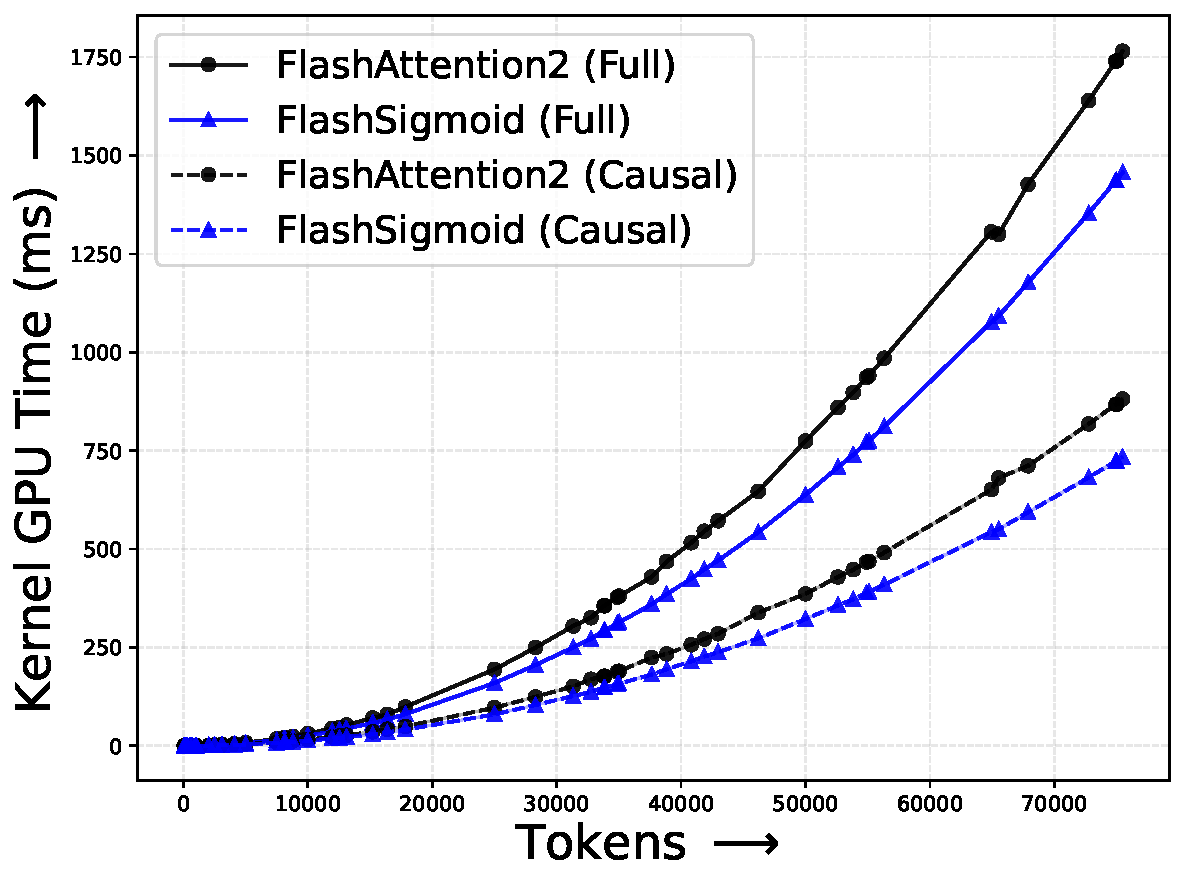
\includegraphics[trim={0 0 0 0}, width=\textwidth]{figures/_flash_figures/final_arxiv/f2/h100/H100_noalibi_FWD_Full_17.39_0.07_Causal_18.76_0.06.pdf}
        \captionsetup{justification=centering}
        \caption*{
            (a) Inference mode kernels on H100.
        }
    \end{minipage}
    \hfill
    \begin{minipage}{0.46\textwidth}
        \centering        
        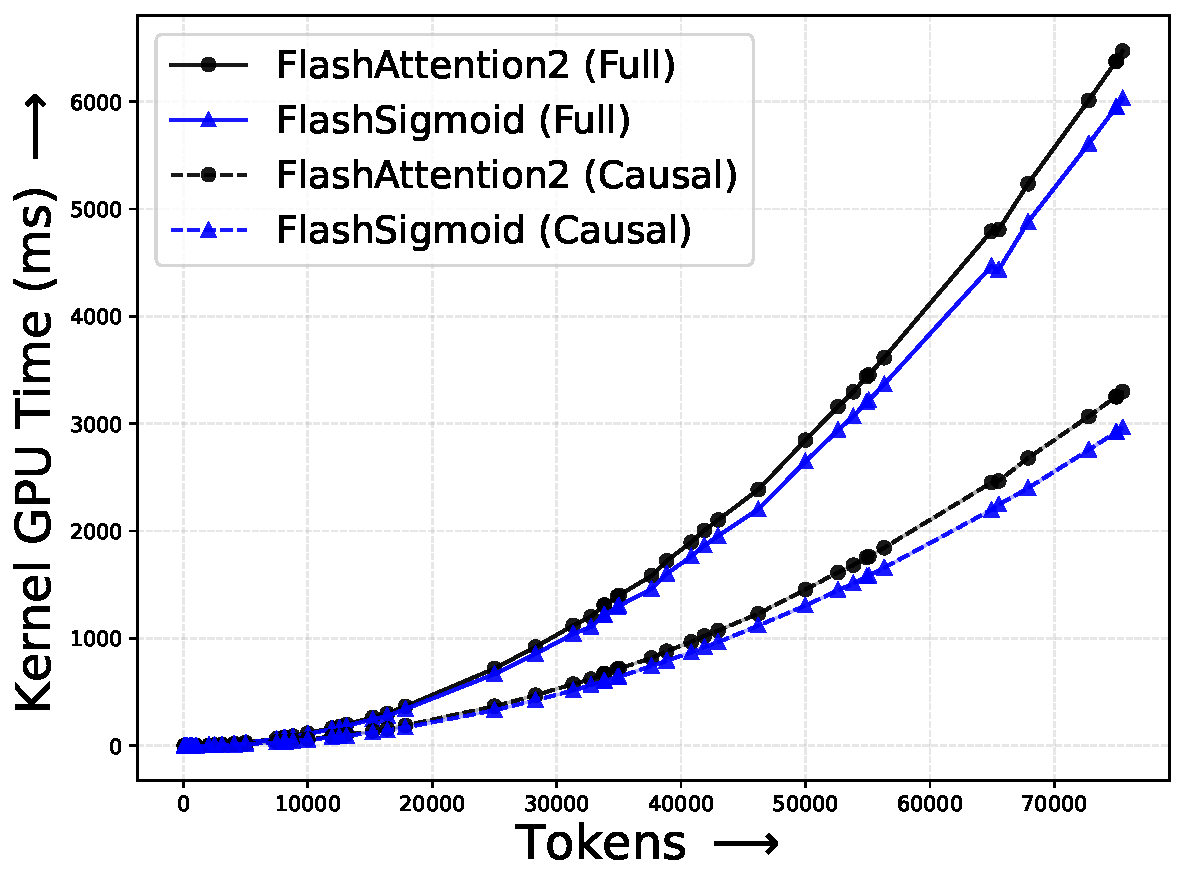
\includegraphics[trim={0 0 0 0}, width=\textwidth]{figures/_flash_figures/final_arxiv/f2/h100/H100_noalibi_FWDBWD_Full_6.53_0.06_Causal_9.46_0.04.pdf}
        \captionsetup{justification=centering} 
        \caption*{
            (b) Training mode kernels on H100.
        }
    \end{minipage}
    \caption{
        On average, for sequence lengths between $[64, 78\mathrm{k}]$, the inference mode kernel of \textsc{FlashSigmoid} is ${17.39}\%$ faster than \textsc{FlashAttention2} for self-attention and ${18.76}\%$ for causal attention.
        The training mode kernels of \textsc{FlashSigmoid} are ${6.53}\%$ faster than \textsc{FlashAttention2} for self-attention and ${9.46}\%$ for causal attention.
        Note that inference involves only the forward pass of the model and training involves both the forward and the backward pass of the model. 
    }
    \label{fig:h100-softmax-sigmoid-fwd-bwd}
\end{figure}
\begin{figure}[!htbp]
    \centering
    \begin{minipage}{0.46\textwidth}
        \footnotesize
        \centering
        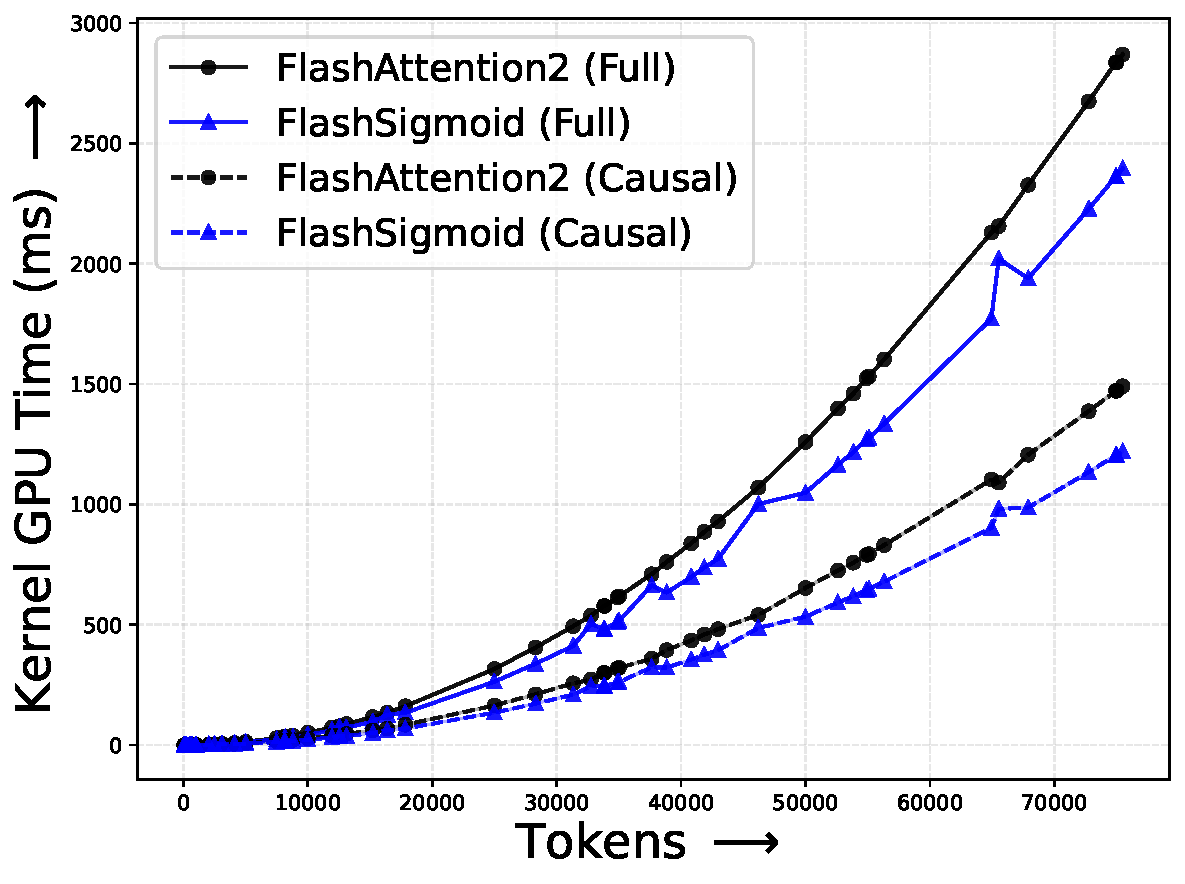
\includegraphics[trim={0 0 0 0}, width=\textwidth]{figures/_flash_figures/final_arxiv/f2/a100/A100_noalibi_FWD_Full_14.33_0.05_Causal_16.92_0.09.pdf}
        \captionsetup{justification=centering}
        \caption*{
            (a) Inference mode kernels on A100.
        }
    \end{minipage}
    \hfill
    \begin{minipage}{0.46\textwidth}
        \centering        
        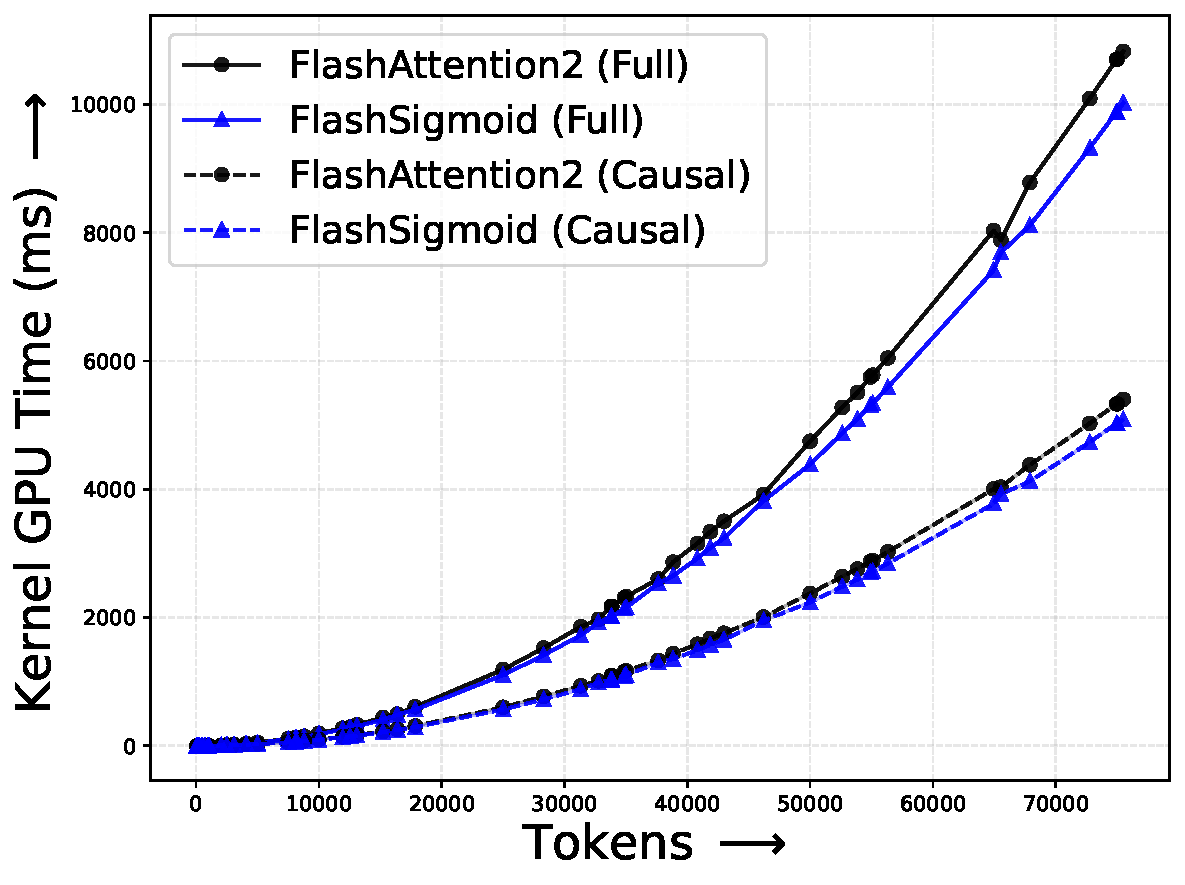
\includegraphics[trim={0 0 0 0}, width=\textwidth]{figures/_flash_figures/final_arxiv/f2/a100/A100_noalibi_FWDBWD_Full_6.02_0.06_Causal_5.27_0.07.pdf}
        \captionsetup{justification=centering} 
        \caption*{
            (b) Training mode kernels on A100.
        }
    \end{minipage}
    \caption{
        On average, for sequence lengths between $[64, 78\mathrm{k}]$, the inference mode kernel of \textsc{FlashSigmoid} is ${14.33}\%$ faster than \textsc{FlashAttention2} for self-attention and ${16.92}\%$ for causal attention.
        The training mode kernels of \textsc{FlashSigmoid} are ${6.02}\%$ faster than \textsc{FlashAttention2} for self-attention and ${5.27}\%$ for causal attention.
        Note that inference involves only the forward pass of the model and training involves both the forward and the backward pass of the model. 
    }
    \label{fig:a100-softmax-sigmoid-fwd-bwd}
\end{figure}
\vspace{-0.1in}

\noindent\textbf{Results:}\ \Cref{fig:h100-softmax-sigmoid-fwd-bwd,fig:a100-softmax-sigmoid-fwd-bwd} show the GPU time comparisons of kernels in inference mode and training mode of \textsc{FlashSigmoid} and \textsc{FlashAttention2} respectively.
We observe that we obtain a large average speed-boost for inference and a modest average speed-boost for training. 
Note that the speed-ups in all the subsequent figures are obtained by averaging the performances for tokens sampled in the range of $[64, 78\mathrm{k}]$.

\noindent \textbf{Details of Individual Kernels:}\ Next, we also show the performance of individual flash kernels of \textsc{FlashSigmoid} and \textsc{FlashAttention2}.
Note that inference mode involves only the forward pas of the model, while training mode involves both the forward and the backward pass of the model.
The forward pass of both these approaches involves one kernel, which we term \textrm{flash\char`_fwd\char`_kernel}, and the backward pass of both these approaches is made up of three kernels, which we term \textrm{bwd\char`_dq\char`_dk\char`_dv}, \textrm{bwd\char`_dot\char`_do\char`_o}, and \textrm{bwd\char`_convert\char`_dq}.
In code, the real names of these kernels are as follows.
\begin{equation}
    \label{eq:KernelRealNames}
    \begin{aligned}
    \textrm{fwd}
    &
    := 
    \textrm{flash\char`_fwd\char`_kernel}
    \\
    \textrm{bwd\char`_dq\char`_dk\char`_dv}
    &
    :=    \textrm{flash\char`_bwd\char`_dq\char`_dk\char`_dv\char`_loop\char`_seqk\char`_parallel\char`_kernel}
    \\
    \textrm{bwd\char`_dot\char`_do\char`_o}
    &
    :=
    \textrm{flash\char`_bwd\char`_dot\char`_do\char`_o\char`_kernel}
    \\
    \textrm{bwd\char`_convert\char`_dq}
    &
    :=
    \textrm{flash\char`_bwd\char`_convert\char`_dq\char`_kernel}
    \end{aligned}    
\end{equation} 
\noindent Here, we first provide a brief description of the tasks performed by each of these kernels; for a detailed explanation, we refer the reader to \textsc{FlashAttention2}~\citep{DBLP:journals/corr/abs-2307-08691} paper and code.
The \textrm{fwd} kernel computes the full forward pass of the model as shown in \cref{table:ComparisonOfForwardBackward}. 
The bulk of computations of the backward pass happen in the \textrm{bwd\char`_dq\char`_dk\char`_dv} kernel, which performs re-computation of attention matrix and reduction of key and value gradient tensors ($\mathbf{d}\mK$, $\mathbf{d}\mV$). 
Again, the exact steps carried out in the backward pass can be checked from \cref{table:ComparisonOfForwardBackward}. 
The \textrm{bwd\char`_convert\char`_dq} kernel performs the reduction of query gradient tensor ($\mathbf{d}\mQ$).
Finally, note that the \textrm{bwd\char`_dot\char`_do\char`_o} kernel in \textsc{FlashAttention2} performs the task of computing the $\textrm{rowsum}(\mathbf{d}\mO\odot \mO)$ tensor along with clearing of the accumulators of query gradients ($\mathbf{d}\mQ$).
Although \textsc{FlashSigmoid} does not require this row-sum tensor, the clearing of accumulators of query gradients is still needed. 
For this reason, \textrm{bwd\char`_dot\char`_do\char`_o} kernel also appears in the profiling of \textsc{FlashSigmoid}.

\noindent \textbf{Performance of Individual Kernels:}\ ~\Cref{fig:h100-softmax-sigmoid-kernels,fig:a100-softmax-sigmoid-kernels} show the performance comparison of each flash kernel in \textsc{FlashSigmoid} with the corresponding kernel in \textsc{FlashAttention2} when tested on an H100 GPU and an A100 GPU respectively.
We observe that on both the H100 and A100 GPU architectures, the \textrm{fwd} kernel of \textsc{FlashSigmoid} is significantly faster than that of \textsc{FlashAttention2} and the \textrm{bwd\char`_dq\char`_dk\char`_dv} kernel of \textsc{FlashSigmoid} has a modest average speed boost over \textsc{FlashAttention2}.
The \textrm{bwd\char`_dot\char`_do\char`_o} kernel in \textsc{FlashSigmoid} is significantly faster on A100 GPUs.
Note that even though the \textrm{bwd\char`_dot\char`_do\char`_o} kernel of \textsc{FlashSigmoid} appears to be slower on average on H100 GPUs, the kernel time of \textrm{bwd\char`_dot\char`_do\char`_o} ($\sim 5$ms) is negligible compared to that of the main \textrm{bwd\char`_dq\char`_dk\char`_dv} kernel ($\sim 5000$ms). 
Thus, the combined backward pass kernel in \textsc{FlashSigmoid} time does not suffer from this slowdown. 
Finally, note that for \textrm{bwd\char`_convert\char`_dq}, \textsc{FlashSigmoid} and \textsc{FlashAttention2} have identical performance.
This is expected, since the task of this kernel is to reduce the gradient of the queries $\mathbf{d}\mQ$, which is a common step in both the approaches and is not modified in \textsc{FlashSigmoid}. 
\begin{figure}[!htbp]
    \centering
    \begin{minipage}{0.24\textwidth}
        \footnotesize
        \centering
        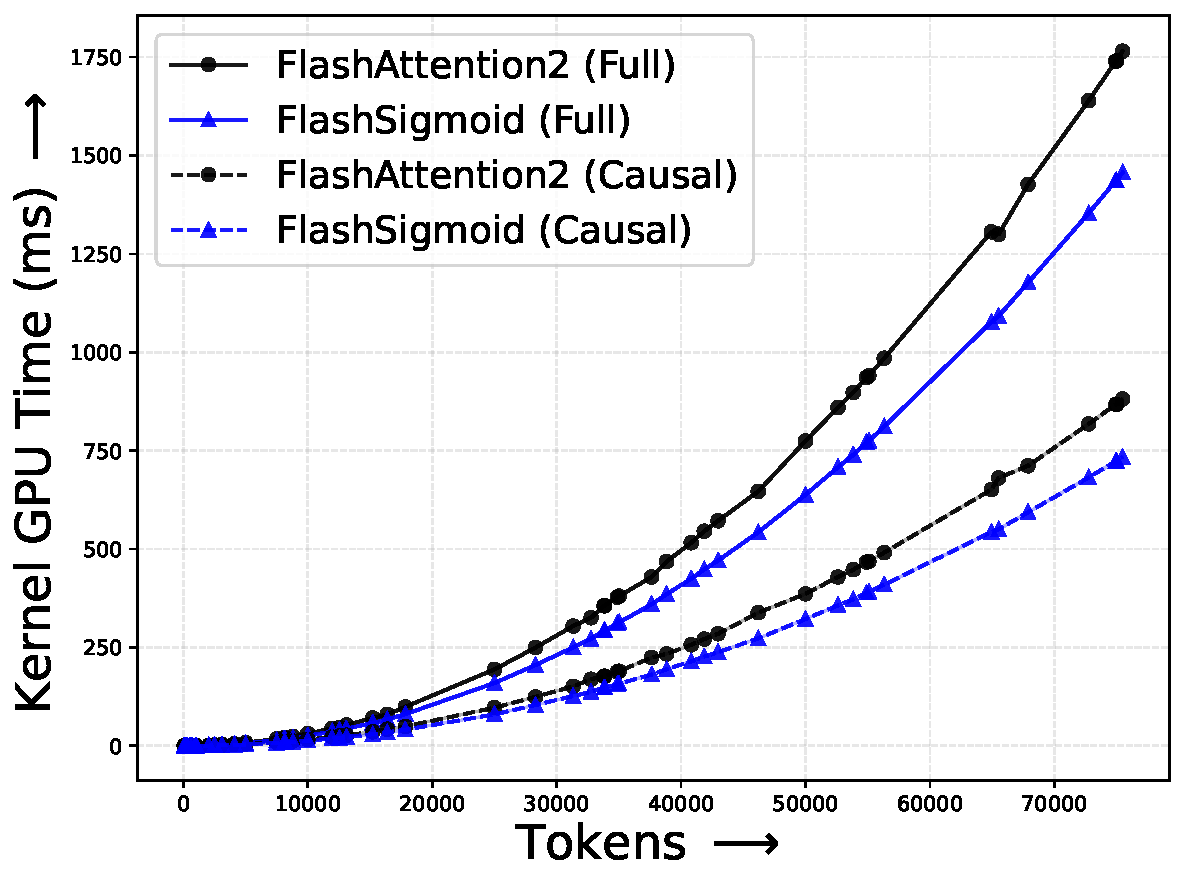
\includegraphics[trim={0 0 0 0}, width=\textwidth]{figures/_flash_figures/final_arxiv/f2/individual/h100/H100_noalibi_flash_fwd_kernel_Full_17.39_0.07_Causal_18.76_0.06.pdf}
        \captionsetup{justification=centering}
        \caption*{
            fwd:\\$17.39\%$ faster for self-attention and $18.76\%$ for causal.
        } 
    \end{minipage}
    \hfill
    \begin{minipage}{0.24\textwidth}
        \centering        
        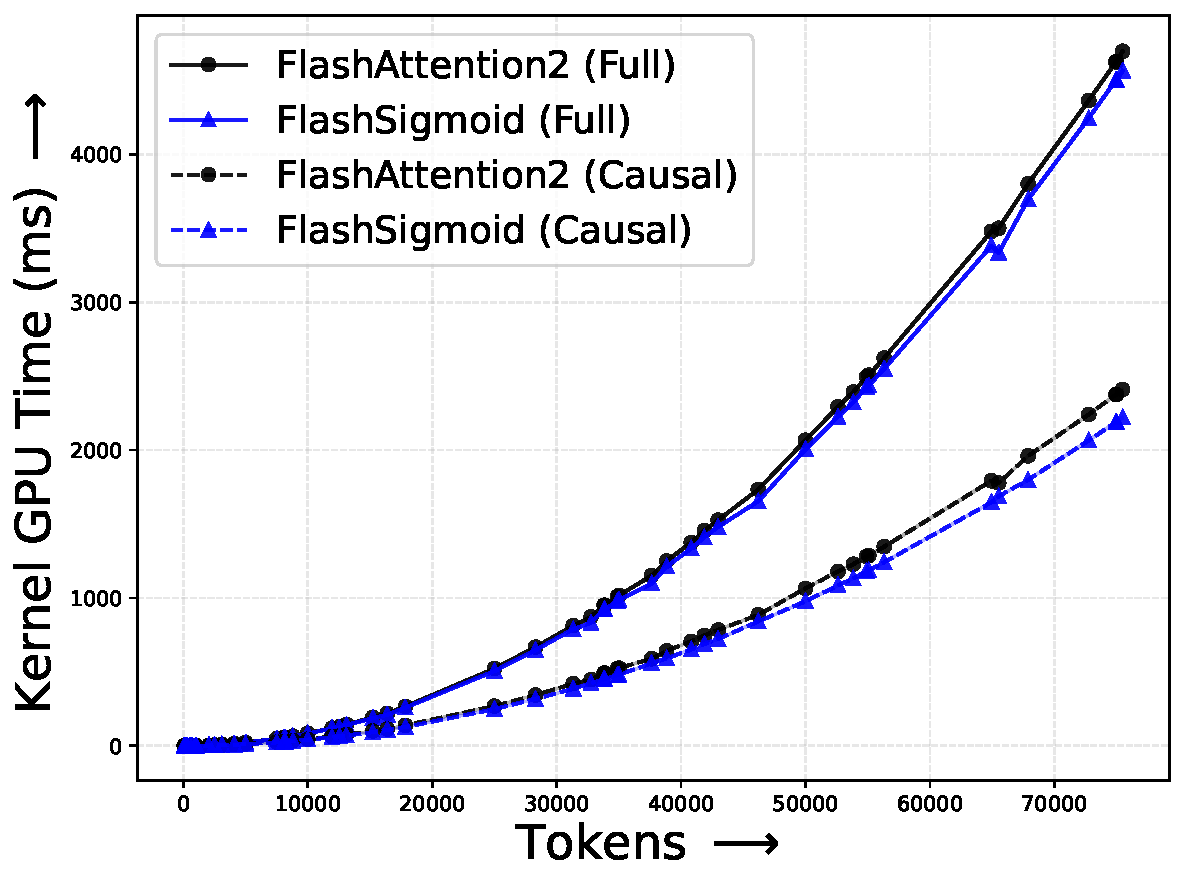
\includegraphics[trim={0 0 0 0}, width=\textwidth]{figures/_flash_figures/final_arxiv/f2/individual/h100/H100_noalibi_flash_bwd_dq_dk_dv_loop_seqk_parallel_kernel_Full_3.29_0.06_Causal_6.97_0.07.pdf}
        \captionsetup{justification=centering} 
        \caption*{
            \textrm{bwd\char`_dq\char`_dk\char`_dv}:\\$3.29\%$ faster for self-attention and $6.97\%$ for causal.
        }
    \end{minipage}
    \hfill
    \begin{minipage}{0.24\textwidth}
        \centering        
        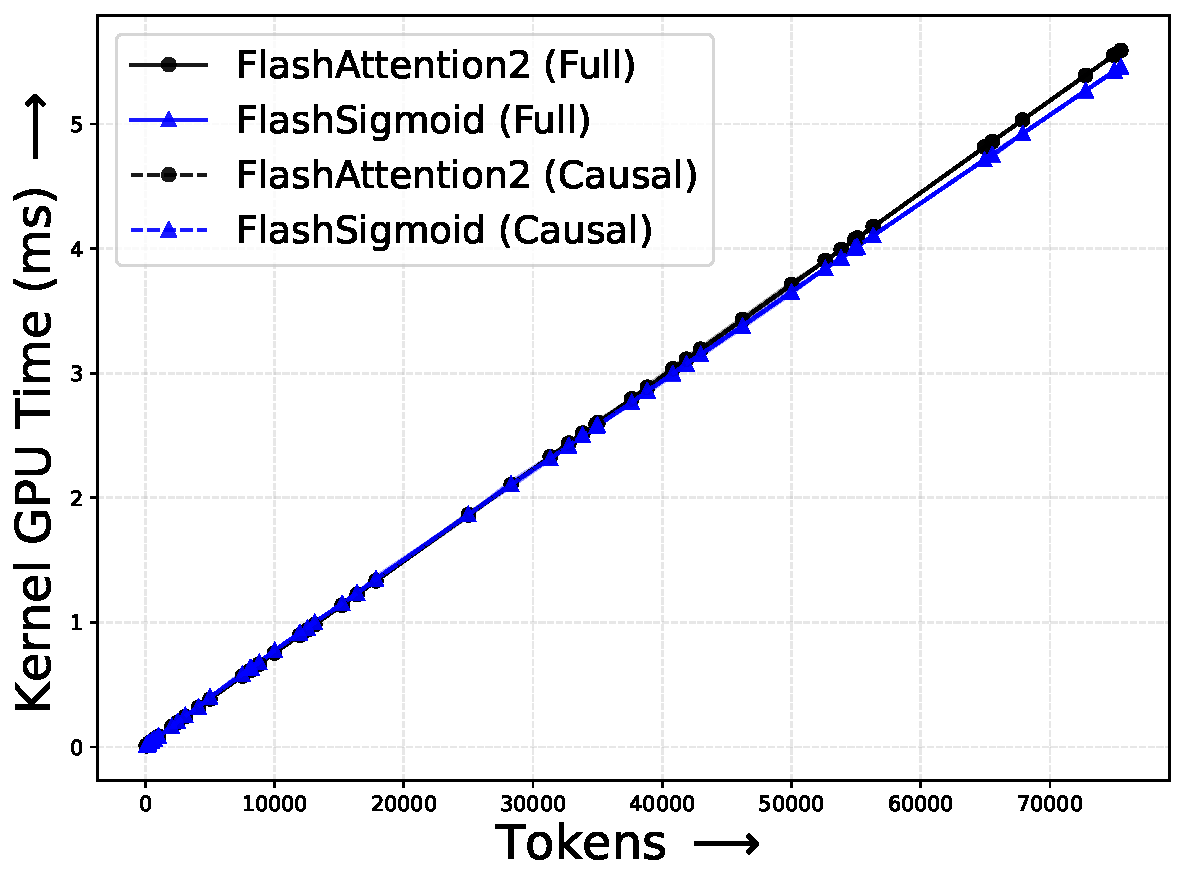
\includegraphics[trim={0 0 0 0}, width=\textwidth]{figures/_flash_figures/final_arxiv/f2/individual/h100/H100_noalibi_flash_bwd_dot_do_o_kernel_Full_-2.24_0.06_Causal_-2.17_0.06.pdf}
        \captionsetup{justification=centering} 
        \caption*{
            \textrm{bwd\char`_dot\char`_do\char`_o}:\\
            $2.24\%$ slower for self-attention and $2.17\%$ for causal.  
        }
    \end{minipage}
    \hfill
    \begin{minipage}{0.24\textwidth}
        \centering        
        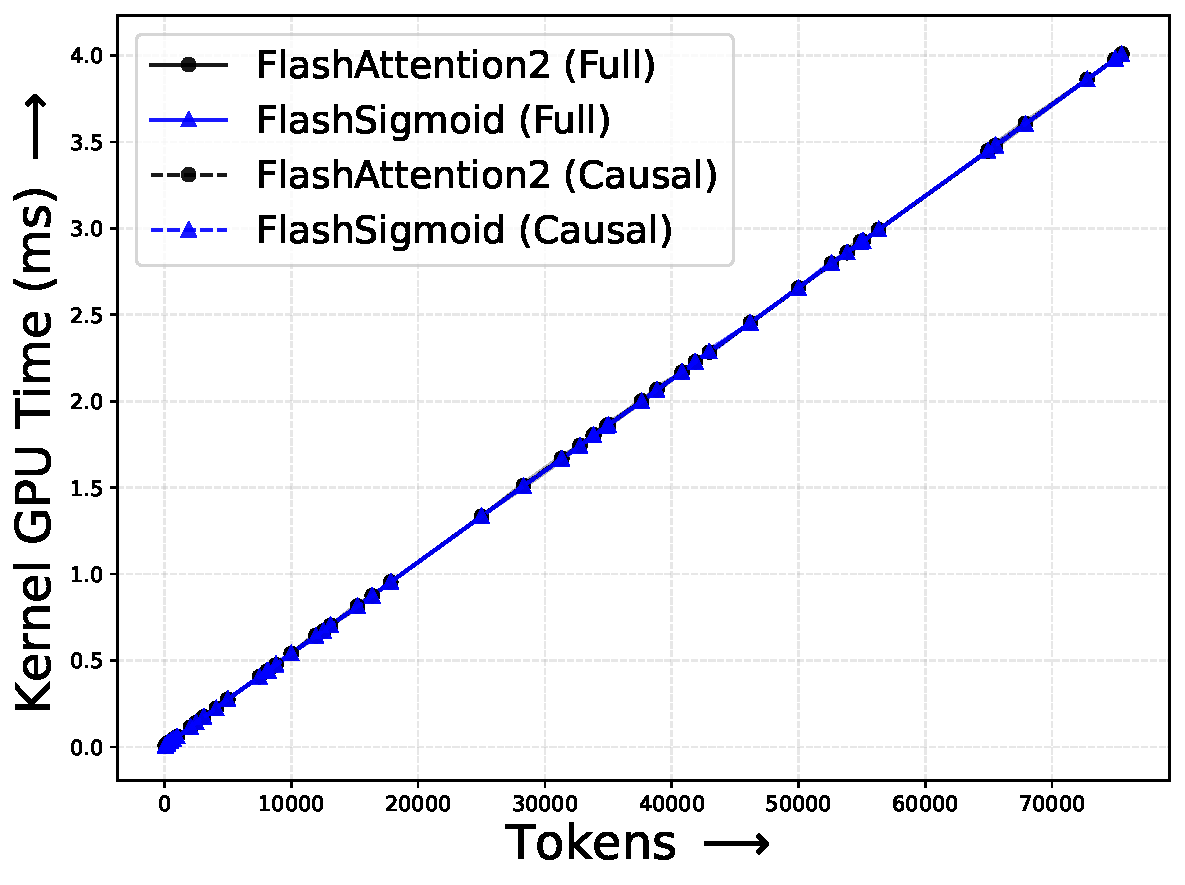
\includegraphics[trim={0 0 0 0}, width=\textwidth]{figures/_flash_figures/final_arxiv/f2/individual/h100/H100_noalibi_flash_bwd_convert_dq_kernel_Full_0.03_0.05_Causal_-0.02_0.04.pdf}
        \captionsetup{justification=centering} 
        \caption*{
            \textrm{bwd\char`_convert\char`_dq}:\\
            $0.03\%$ faster for self-attention, $0.02\%$ slower for causal. 
        }
    \end{minipage}
    \caption{
        \textsc{FlashSigmoid} and \textsc{FlashAttention2} kernel comparison on H100 GPUs. 
    }
    \label{fig:h100-softmax-sigmoid-kernels}
\end{figure}
\begin{figure}[!htbp]
    \centering
    \begin{minipage}{0.24\textwidth}
        \footnotesize
        \centering
        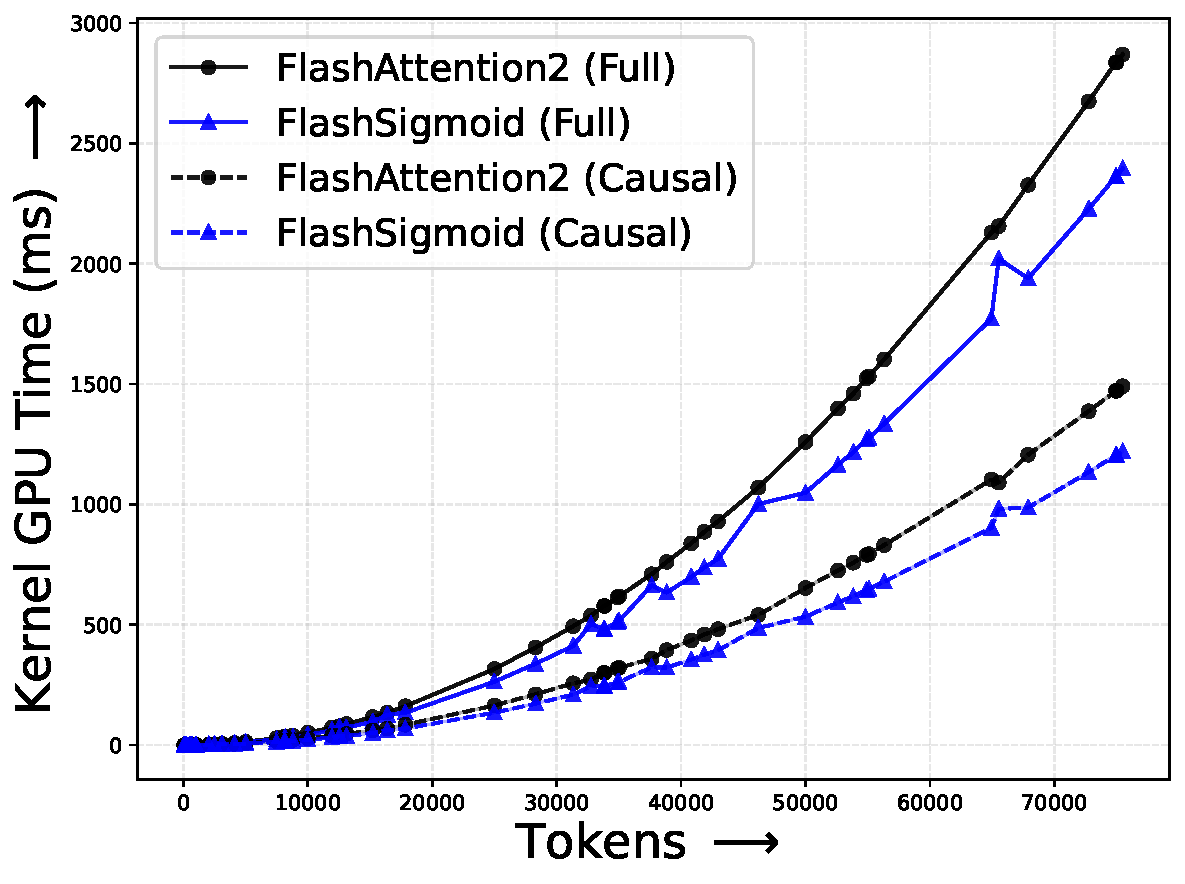
\includegraphics[trim={0 0 0 0}, width=\textwidth]{figures/_flash_figures/final_arxiv/f2/individual/a100/A100_noalibi_flash_fwd_kernel_Full_14.33_0.05_Causal_16.92_0.09.pdf}
        \captionsetup{justification=centering}
        \caption*{
            fwd:\\$14.33\%$ faster for self-attention and $16.92\%$ for causal. 
        } 
    \end{minipage}
    \hfill
    \begin{minipage}{0.24\textwidth}
        \centering        
        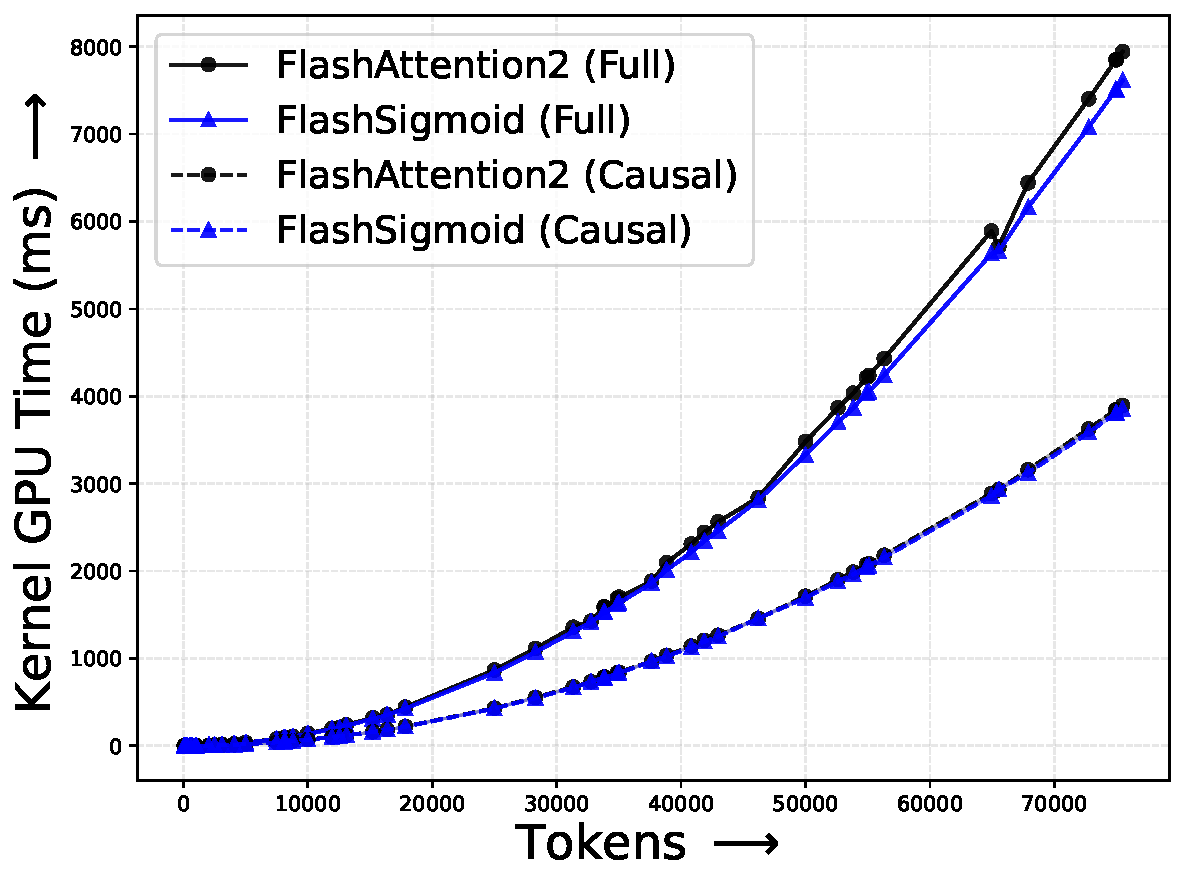
\includegraphics[trim={0 0 0 0}, width=\textwidth]{figures/_flash_figures/final_arxiv/f2/individual/a100/A100_noalibi_flash_bwd_dq_dk_dv_loop_seqk_parallel_kernel_Full_3.5_0.06_Causal_1.39_0.08.pdf}
        \captionsetup{justification=centering} 
        \caption*{
            \textrm{bwd\char`_dq\char`_dk\char`_dv}:\\$3.50\%$ faster for self-attention and $1.39\%$ for causal.
        }
    \end{minipage}
    \hfill
    \begin{minipage}{0.24\textwidth}
        \centering        
        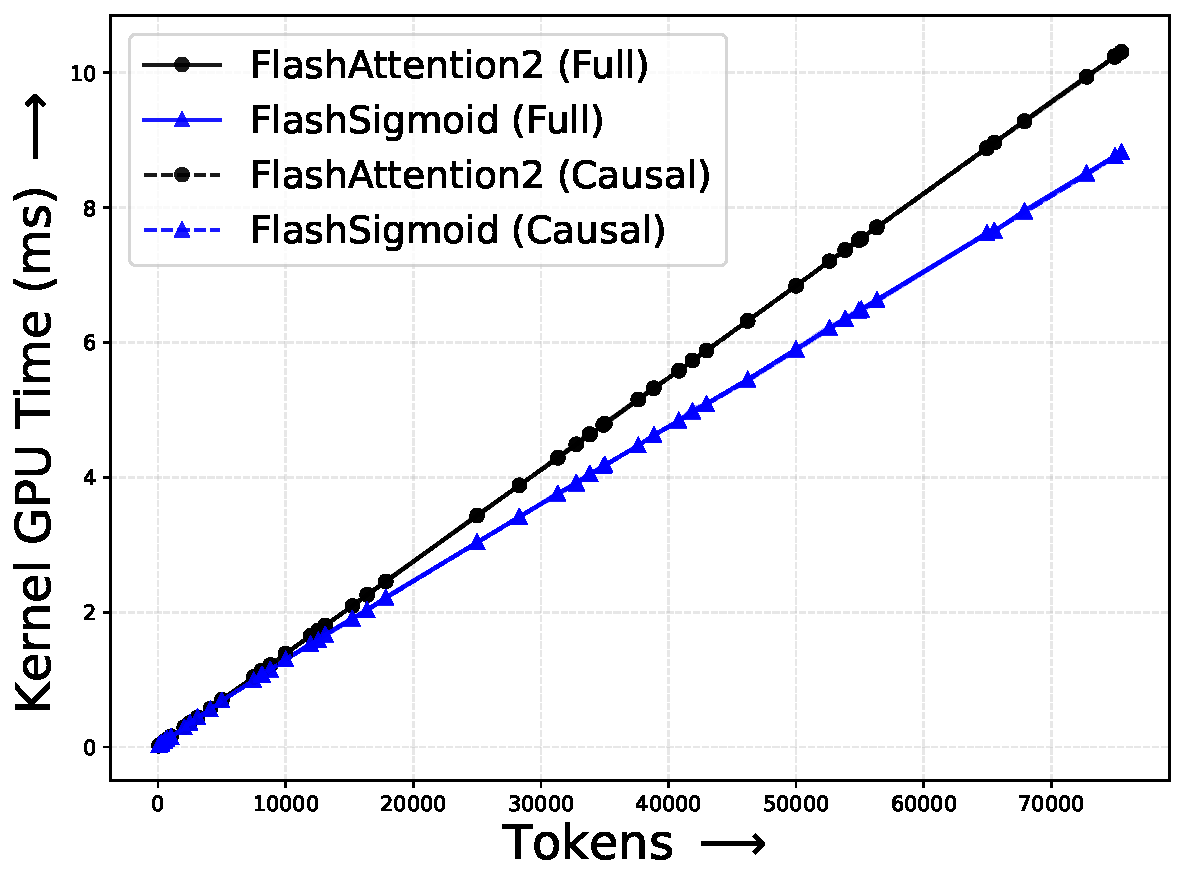
\includegraphics[trim={0 0 0 0}, width=\textwidth]{figures/_flash_figures/final_arxiv/f2/individual/a100/A100_noalibi_flash_bwd_dot_do_o_kernel_Full_7.95_0.34_Causal_8.0_0.35.pdf}
        \captionsetup{justification=centering} 
        \caption*{
            \textrm{bwd\char`_dot\char`_do\char`_o}:\\
            $7.95\%$ faster for self-attention and $8.00\%$ for causal.  
        }
    \end{minipage}
    \hfill
    \begin{minipage}{0.24\textwidth}
        \centering        
        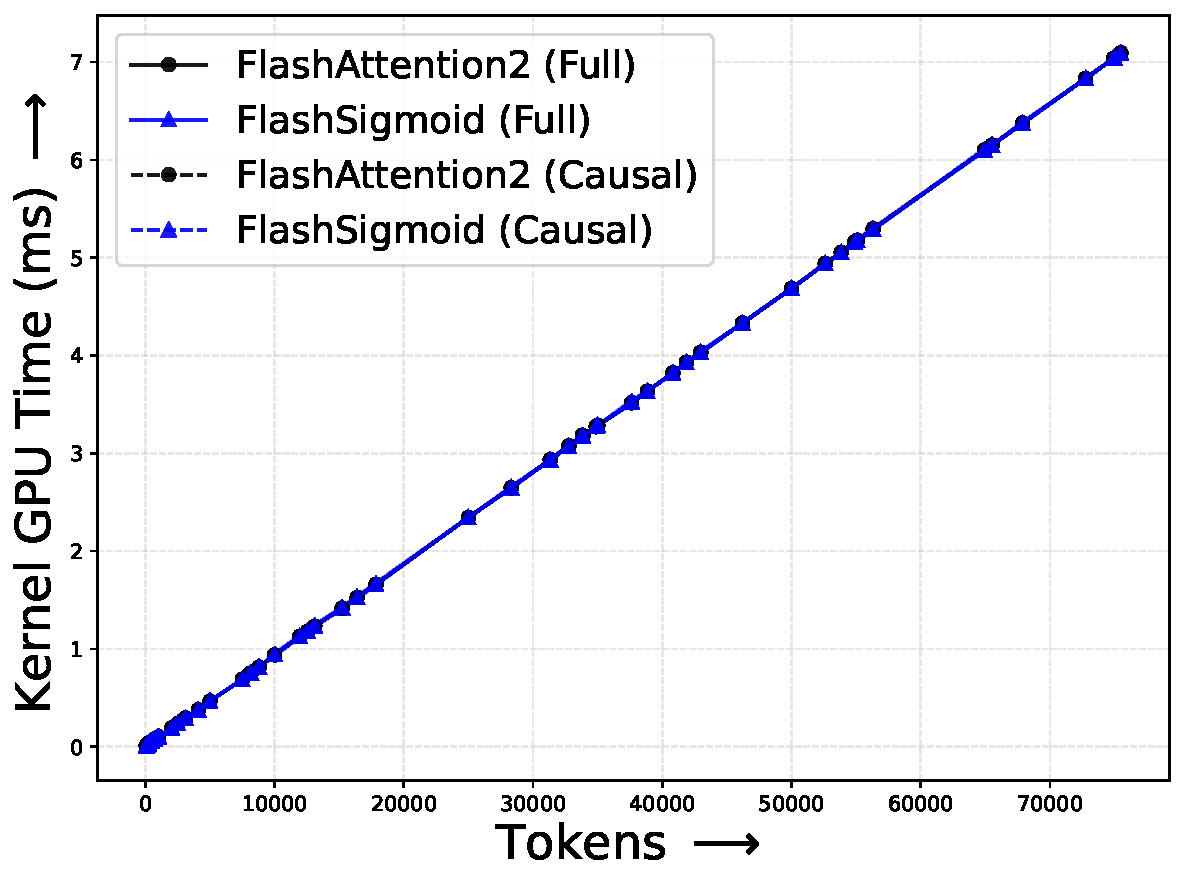
\includegraphics[trim={0 0 0 0}, width=\textwidth]{figures/_flash_figures/final_arxiv/f2/individual/a100/A100_noalibi_flash_bwd_convert_dq_kernel_Full_0.01_0.04_Causal_-0.03_0.04.pdf}
        \captionsetup{justification=centering} 
        \caption*{
            \textrm{bwd\char`_convert\char`_dq}:\\
            $0.01\%$ faster for self-attention, $0.03\%$ slower for causal. 
        }
    \end{minipage}
    \caption{
        \textsc{FlashSigmoid} and \textsc{FlashAttention2} kernel comparison on A100 GPUs. 
    }
    \label{fig:a100-softmax-sigmoid-kernels}
\end{figure}
\subsection{Speed Boosts of \textsc{FlashSigmoid} in Realistic Settings}
\label{sec:SpeedBoostsOfFlashSigmoidInRealisticSettings}
\noindent In this section, we demonstrate how the performance boosts measured in \cref{sec:PerformanceAnalysisOfFlashSigmoidKernels} for the individual kernels of \textsc{FlashSigmoid} contributes to speeding-up realistic runs with end-to-end training. 

\noindent\textbf{Setup:}\ As a target experiment, we consider training a vision transformer~\citep{DBLP:conf/iclr/DosovitskiyB0WZ21} on the ImageNet dataset~\citep{DBLP:conf/cvpr/DengDSLL009}. 
We create two vision transformer model variants-- one with \textsc{FlashAttention2} attention and the other with \textsc{FlashSigmoid} attention. 
We carry out the training of these models with a distributed data-parallel (DDP) setup using PyTorch~\citep{DBLP:conf/nips/PaszkeGMLBCKLGA19}. 
We perform two sets of experiments-- \emph{i.} the first performs DDP training on four nodes of H100 GPUs with eight GPUs per node and EFA/RDMA interconnect for the nodes, and \emph{ii.} the second performs DDP training on four nodes of A100 GPUs with eight GPUs per node. 
In each set of experiments, we use three different image sizes ($64\times 64$, $90\times 90$, and $100\times 100$), along with patch size of $1$ to result in different number of tokens for the underlying attention mechanism in the vision transformer model ($64\times 64 = 4096$, $90\times 90 = 8100$, and $100\times 100 = 10000$ tokens).
For each of these configurations, we select batch sizes so that the GPU memory utilization would be greater than $80\%$.
These considerations are in order to minimize, if not eliminate, other confounders that can unfairly affect estimation speed-ups in realistic runs. For instance, a low GPU utilization would lead to a larger number of updates, which in turn would incur unnecessary delays, variations, and slow-downs due to across-nodes communications.

\noindent\textbf{Results:}\ The results of the runs on H100 nodes and A100 nodes are shown in \cref{fig:ComparisonsOfFlashesOnH100,fig:ComparisonsOfFlashesOnA100} respectively.
There, we show how the kernel GPU times for forward and backward passes vary according to the number of tokens considered, and include the wall-clock time of the end-to-end runs as explained above. 
We observe that the kernel speed-up reflects significantly in the speed-up of inference of the models (during testing) and modestly in the training of the models.
We observe $\sim8\%$ speed-up in wall-clock time of inference and $\sim4\%$ speed-up in wall-clock time of training. 
\begin{table}[htbp]
    \tiny
    \centering
    \begin{sc}
    \resizebox{\columnwidth}{!}{%
    \begin{tabular}{@{\extracolsep{4pt}}ccccccc}
        \toprule
            \multirow{2}{*}{Tokens}
            &
            \multicolumn{3}{c}{Kernel GPU Time Comparison}
            &
            \multicolumn{3}{c}{Full Run Wall-Clock Time Comparison} 
        \\
        \cmidrule{2-4} 
        \cmidrule{5-7} 
            & 
            Kernels
            & 
            \textsc{FlashAttention2} (ms)
            & 
            \textsc{FlashSigmoid} (ms)
            &  
            Mode
            & 
            \textsc{FlashAttention2} (s)
            & 
            \textsc{FlashSigmoid} (s) 
        \\ 
        \toprule
            \multirow{2}{*}{4096} 
            & 
            $\textrm{fwd}$ 
            & 
            $\reading{4.98}{0.01}$ 
            & 
            $\reading{4.17}{0.01}\ \mathbf{\left(-16.31\%\right)}$
            &   
            $\textrm{Inference}$
            & 
            $\reading{11.17}{0.18}$
            & 
            $\reading{10.68}{0.18}\ \mathbf{\left(-4.42\%\right)}$
        \\
        \cmidrule{2-4} 
        \cmidrule{5-7}  
            & 
            $\textrm{fwd} + \textrm{bwd}$  
            &  
            $\reading{19.58}{0.06}$
            & 
            $\reading{18.12}{0.04}\ \mathbf{\left(-7.45\%\right)}$
            &  
            $\textrm{Training}$
            & 
            $\reading{1563.39}{1.30}$
            & 
            $\reading{1521.68}{2.27}\ \mathbf{\left(-2.67\%\right)}$
        \\
        \toprule
            \multirow{2}{*}{8100} 
            & 
            $\textrm{fwd}$ 
            & 
            $\reading{20.46}{0.05}$
            & 
            $\reading{16.73}{0.05}\ \mathbf{\left(-18.22\%\right)}$
            &  
            $\textrm{Inference}$
            & 
            $\reading{28.21}{0.18}$
            & 
            $\reading{25.93}{0.17}\ \mathbf{\left(-8.06\%\right)}$
        \\
        \cmidrule{2-4} 
        \cmidrule{5-7}  
            & 
            $\textrm{fwd} + \textrm{bwd}$  
            & 
            $\reading{77.63}{0.13}$
            & 
            $\reading{72.70}{0.12}\ \mathbf{\left(-6.35\%\right)}$
            & 
            $\textrm{Training}$ 
            & 
            $\reading{4282.75}{2.14}$
            & 
            $\reading{4129.25}{4.14}\ \mathbf{\left(-3.58\%\right)}$
        \\
        \toprule
            \multirow{2}{*}{10000} 
            & 
            $\textrm{fwd}$ 
            & 
            $\reading{31.17}{0.07}$
            & 
            $\reading{25.49}{0.05}\ \mathbf{\left(-18.20\%\right)}$
            &   
            $\textrm{Inference}$
            & 
            $\reading{38.71}{0.19}$
            & 
            $\reading{35.37}{0.17}\ \mathbf{\left(-8.62\%\right)}$
        \\
        \cmidrule{2-4} 
        \cmidrule{5-7}  
            & 
            $\textrm{fwd} + \textrm{bwd}$  
            & 
            $\reading{117.53}{0.13}$
            & 
            $\reading{109.87}{0.12}\ \mathbf{\left(-6.52\%\right)}$
            &   
            $\textrm{Training}$
            & 
            $\reading{5990.72}{2.21}$
            & 
            $\reading{5751.43}{5.77}\ \mathbf{\left(-3.99\%\right)}$
        \\
        \bottomrule
        \\
    \end{tabular}
    }
    \caption{
        \textsc{FlashSigmoid} vs. \textsc{FlashAttention2} on H100 nodes.
        The kernel GPU time for both the approaches is reported in milliseconds and wall-clock times is reported in seconds per epoch. 
    } 
    \label{fig:ComparisonsOfFlashesOnH100}
    \end{sc}
\end{table}
\begin{table}[htbp]
    \tiny
    \centering
    \begin{sc}
    \resizebox{\columnwidth}{!}{%
    \begin{tabular}{@{\extracolsep{4pt}}ccccccc}
        \toprule
            \multirow{2}{*}{Tokens}
            &
            \multicolumn{3}{c}{Kernel GPU Time Comparison}
            &
            \multicolumn{3}{c}{Full Run Wall-Clock Time Comparison} 
        \\
        \cmidrule{2-4} 
        \cmidrule{5-7} 
            & 
            Kernels
            & 
            \textsc{FlashAttention2} (ms)
            & 
            \textsc{FlashSigmoid} (ms)
            &  
            Mode
            & 
            \textsc{FlashAttention2} (s)
            & 
            \textsc{FlashSigmoid} (s) 
        \\ 
        \toprule
            \multirow{2}{*}{4096} 
            & 
            $\textrm{fwd}$ 
            & 
            $\reading{8.32}{0.02}$
            & 
            $\reading{7.84}{0.03}\ \mathbf{\left(-5.79\%\right)}$
            &   
            $\textrm{Inference}$
            & 
            $\reading{19.05}{0.22}$
            & 
            $\reading{18.74}{0.19}\ \mathbf{\left(-1.65\%\right)}$
        \\
        \cmidrule{2-4} 
        \cmidrule{5-7}  
            & 
            $\textrm{fwd} + \textrm{bwd}$  
            &  
            $\reading{31.81}{0.08}$
            & 
            $\reading{31.11}{0.08}\ \mathbf{\left(-2.19\%\right)}$
            &  
            $\textrm{Training}$
            & 
            $\reading{2795.03}{2.35}$
            & 
            $\reading{2769.44}{5.10}\ \mathbf{\left(-0.92\%\right)}$
        \\
        \toprule
            \multirow{2}{*}{8100} 
            & 
            $\textrm{fwd}$ 
            & 
            $\reading{33.65}{0.09}$
            & 
            $\reading{27.92}{0.07}\ \mathbf{\left(-17.04\%\right)}$
            &  
            $\textrm{Inference}$
            & 
            $\reading{47.35}{0.20}$
            & 
            $\reading{44.05}{0.17}\ \mathbf{\left(-6.96\%\right)}$
        \\
        \cmidrule{2-4} 
        \cmidrule{5-7}  
            & 
            $\textrm{fwd} + \textrm{bwd}$  
            & 
            $\reading{128.18}{0.13}$
            & 
            $\reading{119.04}{0.12}\ \mathbf{\left(-7.13\%\right)}$
            & 
            $\textrm{Training}$ 
            & 
            $\reading{7519.64}{4.21}$
            & 
            $\reading{7254.84}{12.64}\ \mathbf{\left(-3.52\%\right)}$
        \\
        \toprule
            \multirow{2}{*}{10000} 
            & 
            $\textrm{fwd}$ 
            & 
            $\reading{51.17}{0.07}$
            & 
            $\reading{42.49}{0.06}\ \mathbf{\left(-16.96\%\right)}$
            &   
            $\textrm{Inference}$
            & 
            $\reading{64.61}{0.32}$
            & 
            $\reading{59.55}{0.18}\ \mathbf{\left(-7.82\%\right)}$
        \\
        \cmidrule{2-4} 
        \cmidrule{5-7}  
            & 
            $\textrm{fwd} + \textrm{bwd}$  
            & 
            $\reading{194.54}{0.14}$
            & 
            $\reading{180.59}{0.15}\ \mathbf{\left(-7.17\%\right)}$
            &   
            $\textrm{Training}$
            & 
            $\reading{10455.64}{8.85}$
            & 
            $\reading{10052.04}{18.87}\ \mathbf{\left(-3.86\%\right)}$
        \\
        \bottomrule
        \\
    \end{tabular}
    }
    \caption{
        \textsc{FlashSigmoid} vs. \textsc{FlashAttention2} on A100 nodes.
        The kernel GPU time for both the approaches is reported in milliseconds and wall-clock times is reported in seconds per epoch. 
    } 
    \label{fig:ComparisonsOfFlashesOnA100}
    \end{sc}
\end{table}

\noindent\textbf{Connection of Wall-Clock Time Speed-Up and Kernel Speed-Up:}\ 
From \cref{fig:ComparisonsOfFlashesOnA100,fig:ComparisonsOfFlashesOnH100}, it is clear that the speed-up in kernels is larger than that in the wall-clock times of the full runs.
In fact, the speed-up in kernels is the upper bound for the speed-up that we would see in wall-clock times.
To see why, let us denote by $\tau_{\textrm{sm}}$ and $\tau_{\sigma}$ the total kernel GPU time for softmax attention and sigmoid attention respectively. 
Then, the kernel speed-up is given by $s_{\textrm{kernel}} := 1 -  \frac{\tau_{\sigma}}{\tau_{\textrm{sm}}}$. 
However, in a full run, the total wall clock time also incorporates the time required to load data, time taken by other layers of the underlying models, time required to communicate gradients and other data across GPUs and across nodes, and so on.
For our corresponding sigmoid and softmax runs, these extra factors are designed to add, upon expectation, in the same extra time $\tau$.
Thus, the wall-clock time speed-up of a full run with end-to-end training is $s_{\textrm{wall-clock}} := 1 - \frac{\tau_{\sigma} + \tau}{\tau_{\textrm{sm}} + \tau}$. 
Since we have faster sigmoid kernels, we have $\tau_\sigma < \tau_{\textrm{sm}}$, which in turn shows that $s_{\textrm{wall-clock}} = 1 - \frac{\tau_{\sigma} + \tau}{\tau_{\textrm{sm}} + \tau} <  1 -  \frac{\tau_{\sigma}}{\tau_{\textrm{sm}}} = s_{\textrm{kernel}}$. 
This explains the speed boost trends in kernel time versus full run wall-clock time for each setting in \cref{fig:ComparisonsOfFlashesOnA100,fig:ComparisonsOfFlashesOnH100}. 
However, in particular, if a model performs attention mechanism over large number of tokens, the attention mechanism, and hence the corresponding kernel time, starts to dominate the other computations in the network. 
In that case, we see that the wall-clock time speed-boost is closer to the kernel speed-boost.
Mathematically, if $\tau_{\sigma}, \tau_{\textrm{sm}} >\!\!> \tau$, we have: $\tau_{\sigma} + \tau\approx \tau_{\sigma}$, $\tau_{\textrm{sm}} + \tau\approx \tau_{\textrm{sm}}$. 
Thus, $s_{\textrm{kernel}}\approx s_{\textrm{wall-clock}}$, thereby making ${s_{\textrm{wall-clock}}}/{s_{\textrm{kernel}}}\rightarrow 1$. 


\begin{figure}[!htbp]
    \centering
    \begin{minipage}{0.46\textwidth}
        \footnotesize
        \centering
        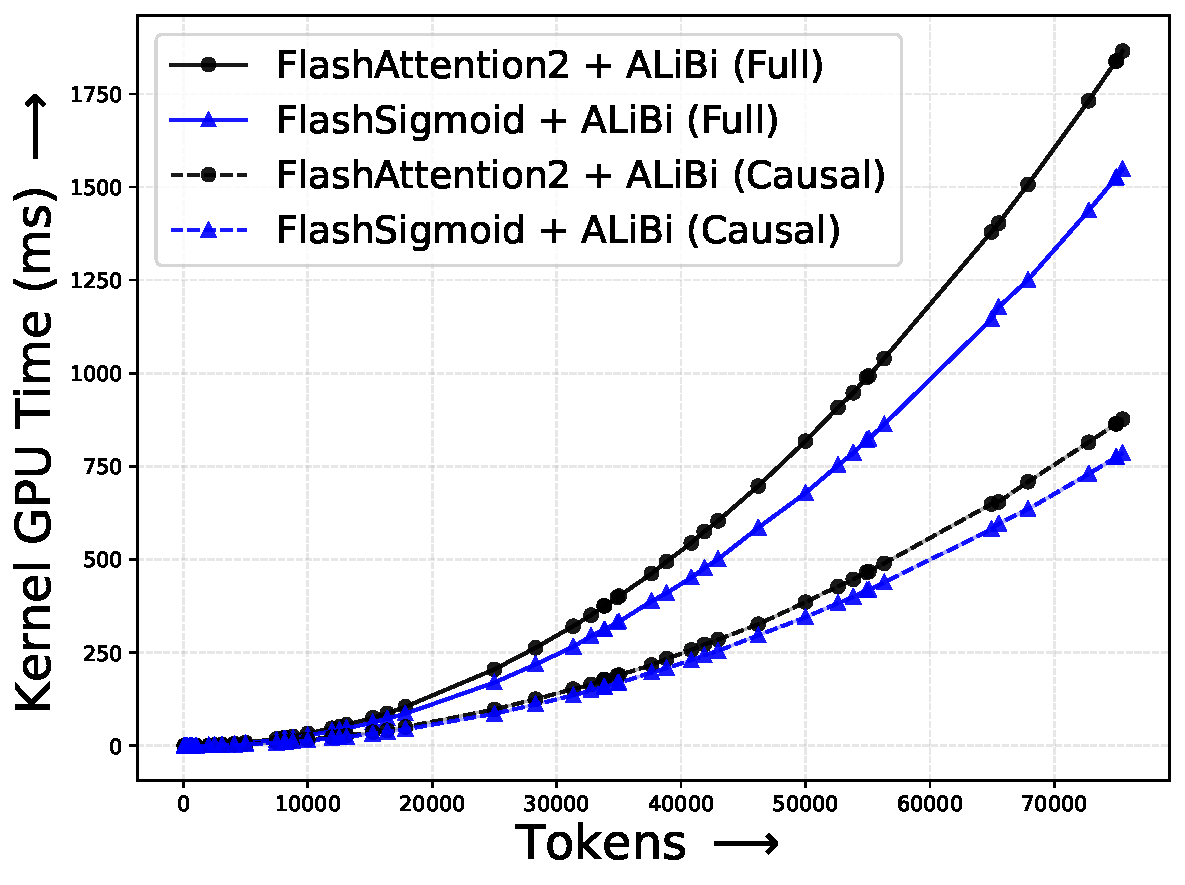
\includegraphics[trim={0 0 0 0}, width=\textwidth]{figures/_flash_figures/final_arxiv/f4/h100/H100_alibi_FWD_Full_17.04_0.04_Causal_10.87_0.24.pdf}
        \captionsetup{justification=centering}
        \caption*{
            (a) Inference mode kernels on H100. 
        }
    \end{minipage}
    \hfill
    \begin{minipage}{0.46\textwidth}
        \centering        
        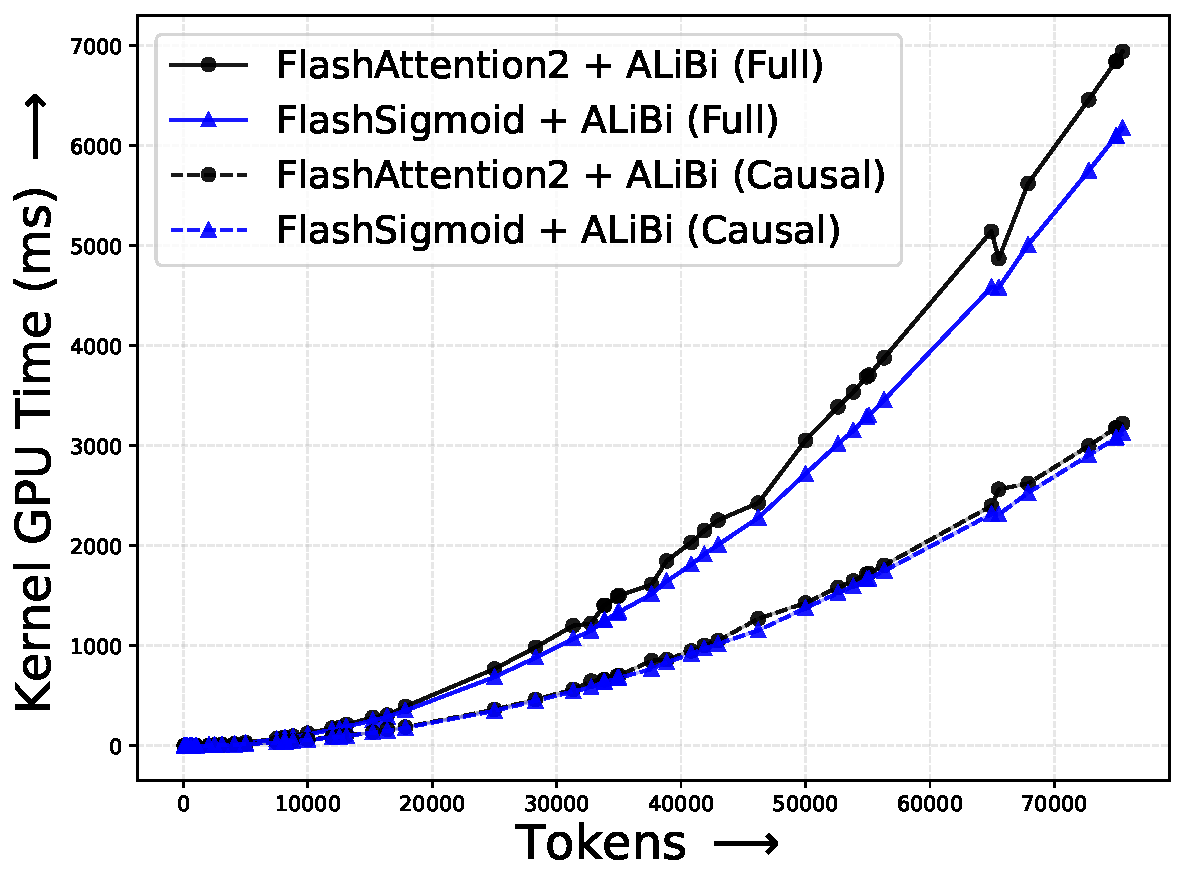
\includegraphics[trim={0 0 0 0}, width=\textwidth]{figures/_flash_figures/final_arxiv/f4/h100/H100_alibi_FWDBWD_Full_8.91_0.05_Causal_4.72_0.1.pdf}
        \captionsetup{justification=centering} 
        \caption*{
            (b) Training mode kernels on H100. 
        }
    \end{minipage}
    \caption{
        On average, for sequence lengths between $[64, 78\mathrm{k}]$, the inference mode kernel of \textsc{FlashSigmoid} is ${17.04}\%$ faster than \textsc{FlashAttention2} for self-attention and ${10.87}\%$ for causal attention.
        The training mode kernels of \textsc{FlashSigmoid} are ${8.91}\%$ faster than \textsc{FlashAttention2} for self-attention and ${4.72}\%$ for causal attention.
        Note that inference involves only the forward pass of the model and training involves both the forward and the backward pass of the model.
    }
    \label{fig:h100-softmax_alibi-sigmoid_alibi-fwd_bwd}
\end{figure}
\begin{figure}[!htbp]
    \centering
    \begin{minipage}{0.46\textwidth}
        \footnotesize
        \centering
        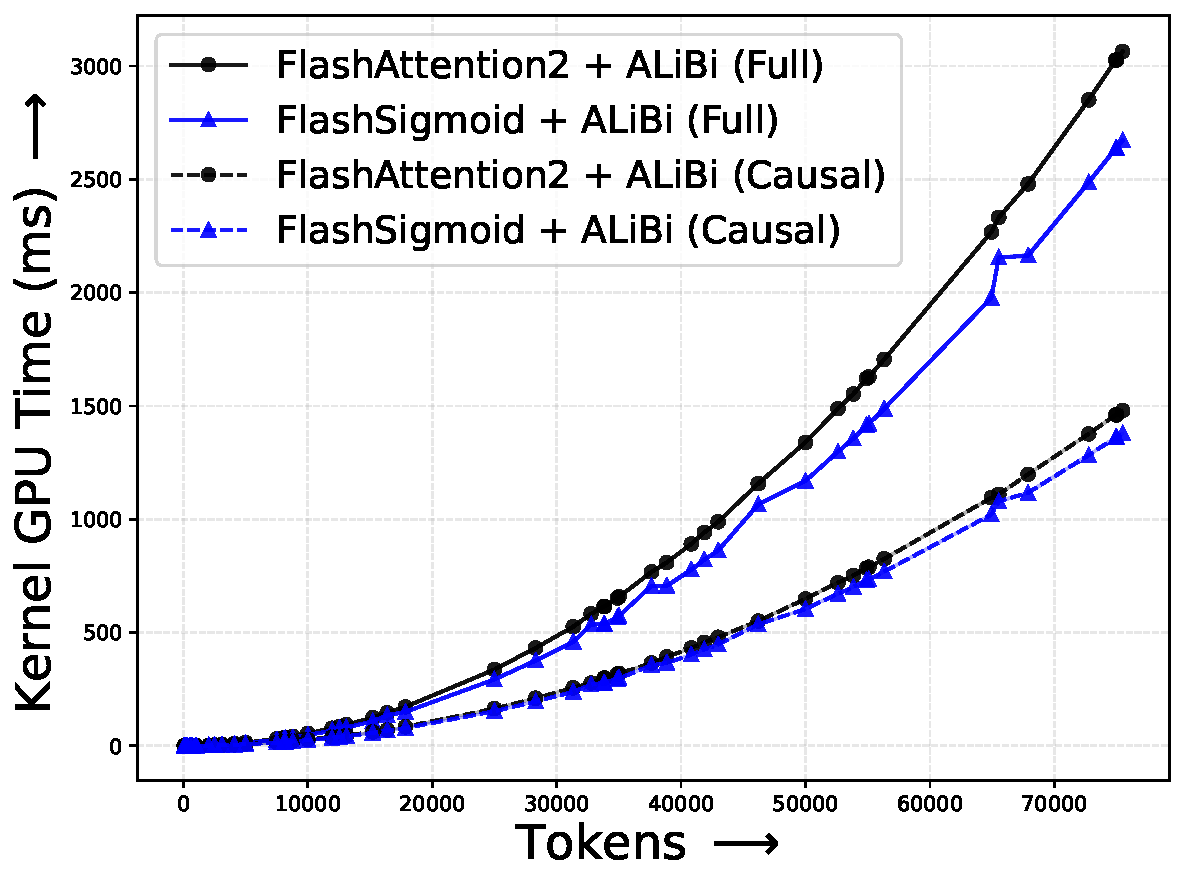
\includegraphics[trim={0 0 0 0}, width=\textwidth]{figures/_flash_figures/final_arxiv/f4/a100/A100_alibi_FWD_Full_12.28_0.1_Causal_5.3_0.07.pdf}
        \captionsetup{justification=centering}
        \caption*{
            (a) Inference mode kernels on A100. 
        }
    \end{minipage}
    \hfill
    \begin{minipage}{0.46\textwidth}
        \centering        
        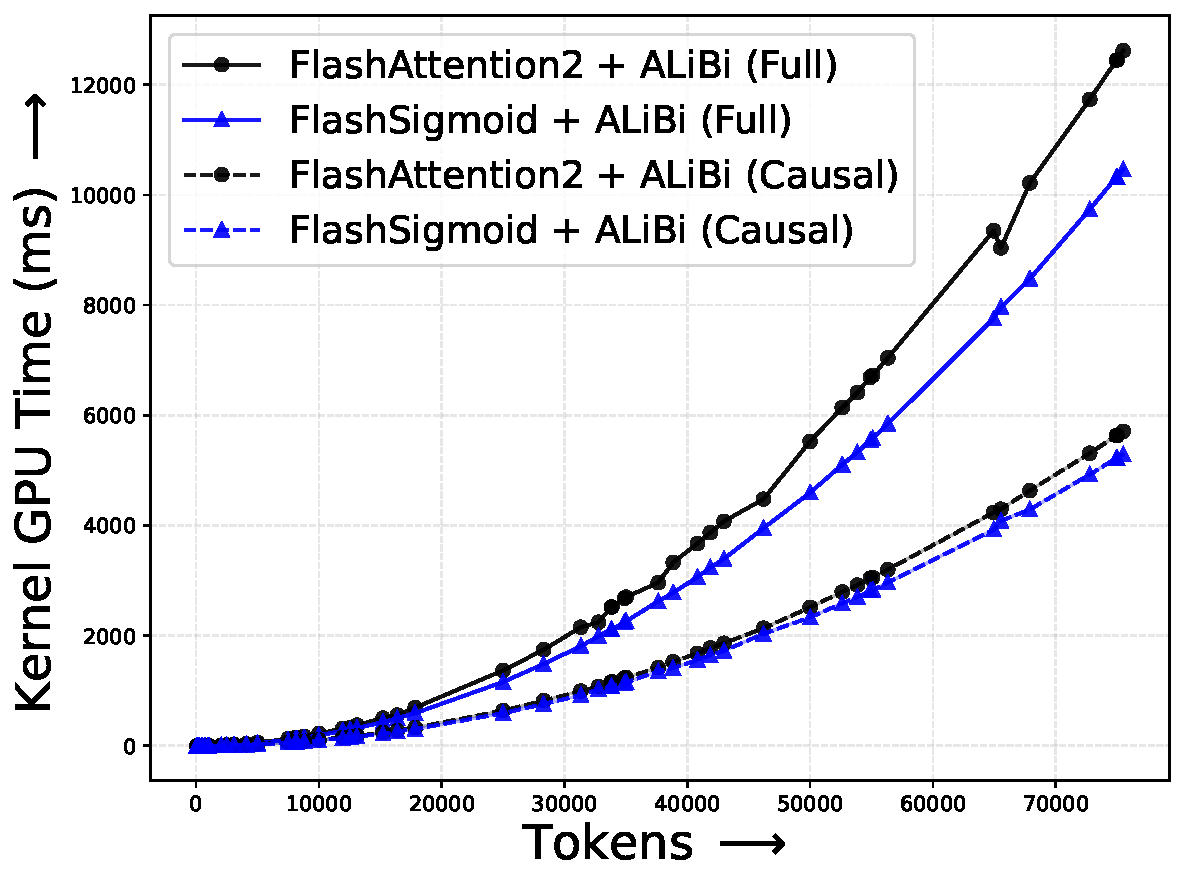
\includegraphics[trim={0 0 0 0}, width=\textwidth]{figures/_flash_figures/final_arxiv/f4/a100/A100_alibi_FWDBWD_Full_14.64_0.08_Causal_6.8_0.03.pdf}
        \captionsetup{justification=centering} 
        \caption*{
            (b) Training mode kernels on A100. 
        }
    \end{minipage}
    \caption{
        On average, for sequence lengths between $[64, 78\mathrm{k}]$, the inference mode kernel of \textsc{FlashSigmoid} is ${12.28}\%$ faster than \textsc{FlashAttention2} for self-attention and ${5.30}\%$ for causal attention.
        The training mode kernels of \textsc{FlashSigmoid} are ${14.64}\%$ faster than \textsc{FlashAttention2} for self-attention and ${6.80}\%$ for causal attention.
        Note that inference involves only the forward pass of the model and training involves both the forward and the backward pass of the model.
    }
    \label{fig:a100-softmax_alibi-sigmoid_alibi-fwd_bwd}
\end{figure}


\noindent\textbf{Significance of Wall-Clock Speed-Up of Inference:}\ Although \textsc{FlashSigmoid} provides only modest gains during training, the speed-up in inference is significant ($> 15\%$ for underlying kernels and $5-10\%$ during inference of full runs).
We posit that this speed-up in inference is extremely critical as well.
Contemporary large-scale models, once trained, spend a huge portion of the rest their lifetime in inference mode~\citep{DBLP:journals/corr/abs-2303-08774}. 
Thus, significant performance boosts in inference mode have immense potential for saving resources in deployment of large models for inference. 

\vspace{-0.1in}
\subsection{\textsc{FlashSigmoid} with ALiBi}
\label{sec:FlashSigmoidWithALiBi}

\noindent It is evident from the main text of the paper that improved positional embeddings, like ALiBi~\citep{DBLP:conf/iclr/PressSL22}, can be crucial for certain tasks and data modalities. 
Thus, we also provide a \textsc{FlashSigmoid} implementation that incorporates ALiBi.
We compare the \textsc{FlashSigmoid} with ALiBi implementation with the \textsc{FlashAttention2} with ALiBi implementation~\citep{DBLP:journals/corr/abs-2307-08691}.
\Cref{fig:a100-softmax_alibi-sigmoid_alibi-fwd_bwd,fig:h100-softmax_alibi-sigmoid_alibi-fwd_bwd} show the kernel GPU time for the forward and backward pass kernels of \textsc{FlashSigmoid} with ALiBi implementation versus \textsc{FlashAttention2} with ALiBi implementation.
Again, we observe that \textsc{FlashSigmoid} kernels for inference have significant speed-up in wall-clock time over those in \textsc{FlashAttention2} and the kernels for training also have modest wall-clock improvements. 






\subsection{Directions for Future Work on \textsc{FlashSigmoid}}
\label{sec:DirectionsForFutureWorkOnFlashSigmoid}
\noindent In this section, we discussed \textsc{FlashSigmoid}, a hardware-aware implementation of the $\sigmoidattn$ algorithm. Then, we demonstrated via kernel benchmarking and realistic setting runs that \textsc{FlashSigmoid} provides significant gains in inference as well as modest gains in training of models with attention mechanism. 
In this subsection we further discuss additional avenues for improving the implementation of \textsc{FlashSigmoid}, and point out some interesting directions for future work.


\noindent\textbf{Optimization of Block Shapes for Different Input and GPU Settings:}\ 
As stated before, our \textsc{FlashSigmoid} implementation builds on \textsc{FlashAttention2} by adding functionality for forward and backward pass of sigmoid attention in place of the standard softmax attention.
In particular, for all \textsc{FlashSigmoid} results discussed so far, we inherit directly from \textsc{FlashAttention2} the details of optimal block shapes, grid shapes, and other kernel launch parameters, and keep them unchanged in our implementation.
For instance, this is the case for the block sizes $B _r, B_c$ in~\cref{alg:FlashSigmoidForward,alg:FlashSigmoidBackward}, which are identical in \textsc{FlashAttention2} and \textsc{FlashSigmoid}.
This choice is dictated by the need to ensure a fair comparison between the two implementations, and allows us to demonstrate the speed-up of sigmoid attention by minimizing confounders associated with parallel computations on different GPU architectures for different input shapes. 

\noindent Although \textsc{FlashSigmoid} kernels lead to speed-ups in inference and training for both H100 and A100 GPUs, we observe that the kernel timing speed-ups on A100 are not uniform across sequence lengths: for a small subset of these, our kernel provides significantly lower speed-up compared to the overall trend for other sequence lengths.
Ideally, the implementation of attention mechanisms should not assume any information on the token count in input, and it is then desirable to have uniform speed-ups across all input lengths. 
Here, we show that this is achievable by simply updating the block shape information in \textsc{FlashSigmoid} to values that are different than those in \textsc{FlashAttention2}. 


\noindent Note that the implementation of \textsc{FlashAttention2} is templated according to block shapes, grid shapes, and other kernel launch parameters.


\noindent Note that \textsc{FlashAttention2} provides various tailored implementations, optimized for different input shapes (e.g., different ranges of feature dimension per head), input types (e.g., causal attention vs. self-attention, ALiBi vs. no ALiBi in attention, etc.), and GPU types (e.g., A100 vs. H100 via checking shared memory size on GPUs). This is achieved by opportunely selecting the kernel template parameters defining block shapes, grid shapes, and other kernel launch parameters for parallel computation on GPUs. 
In our case, we create a variant of \textsc{FlashSigmoid}, denoted by $\textsc{FlashSigmoid}^{\dagger}$, where we update the block sizes for query and key tensors from $\left(B_r, B_c\right) = \left(128, 128\right)$ of \textsc{FlashSigmoid} to $\left(B_r, B_c\right) = \left(128, 64\right)$ of $\textsc{FlashSigmoid}^{\dagger}$ \emph{only} for our input setting (template with features per head being $64$). 
\begin{figure}[!htbp]
    \centering
    \begin{minipage}{0.46\textwidth}
        \footnotesize
        \centering
        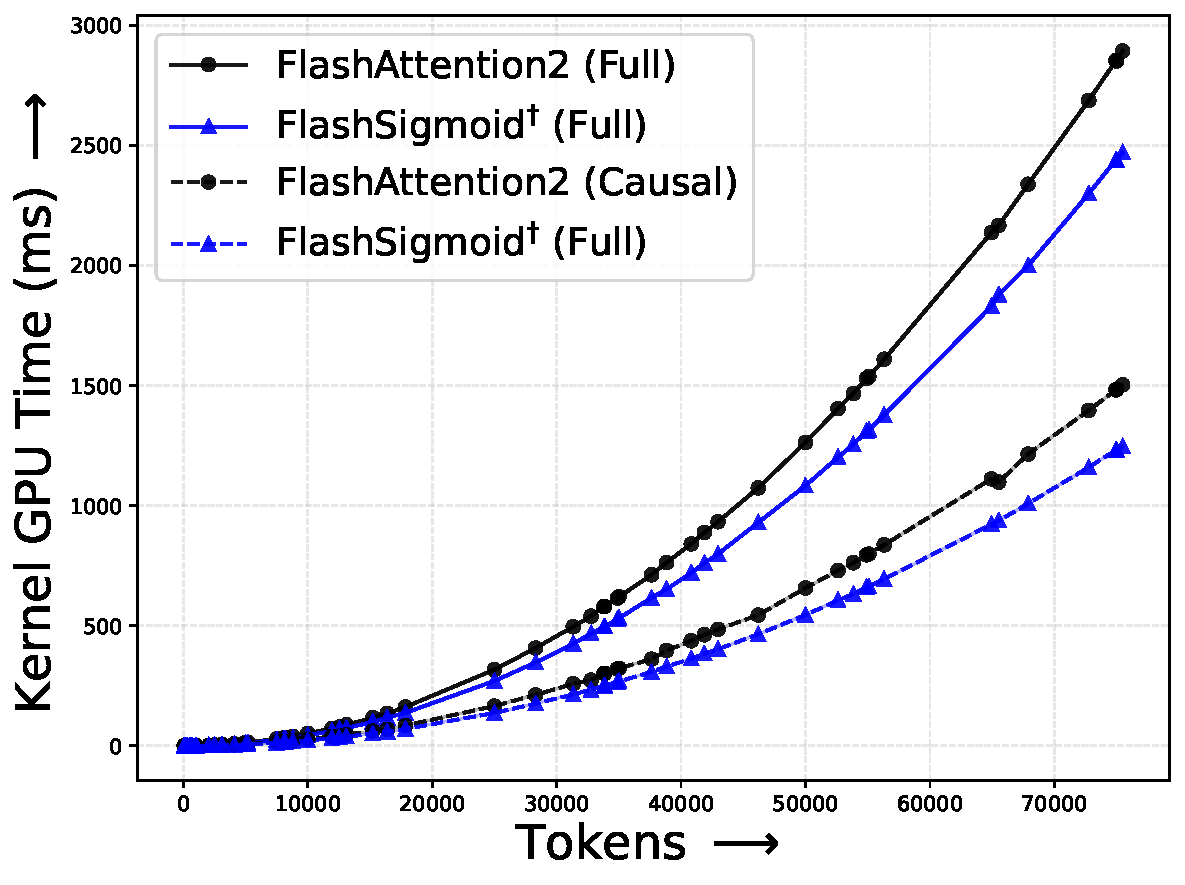
\includegraphics[trim={0 0 0 0}, width=\textwidth]{figures/_flash_figures/final_arxiv/f5/A100_noalibi_FWD_Full_14.82_0.08_Causal_18.02_0.05.pdf}
        \captionsetup{justification=centering}
        \caption*{
            (a) Inference mode kernels on A100.
        }
    \end{minipage}
    \hfill
    \begin{minipage}{0.46\textwidth}
        \centering        
        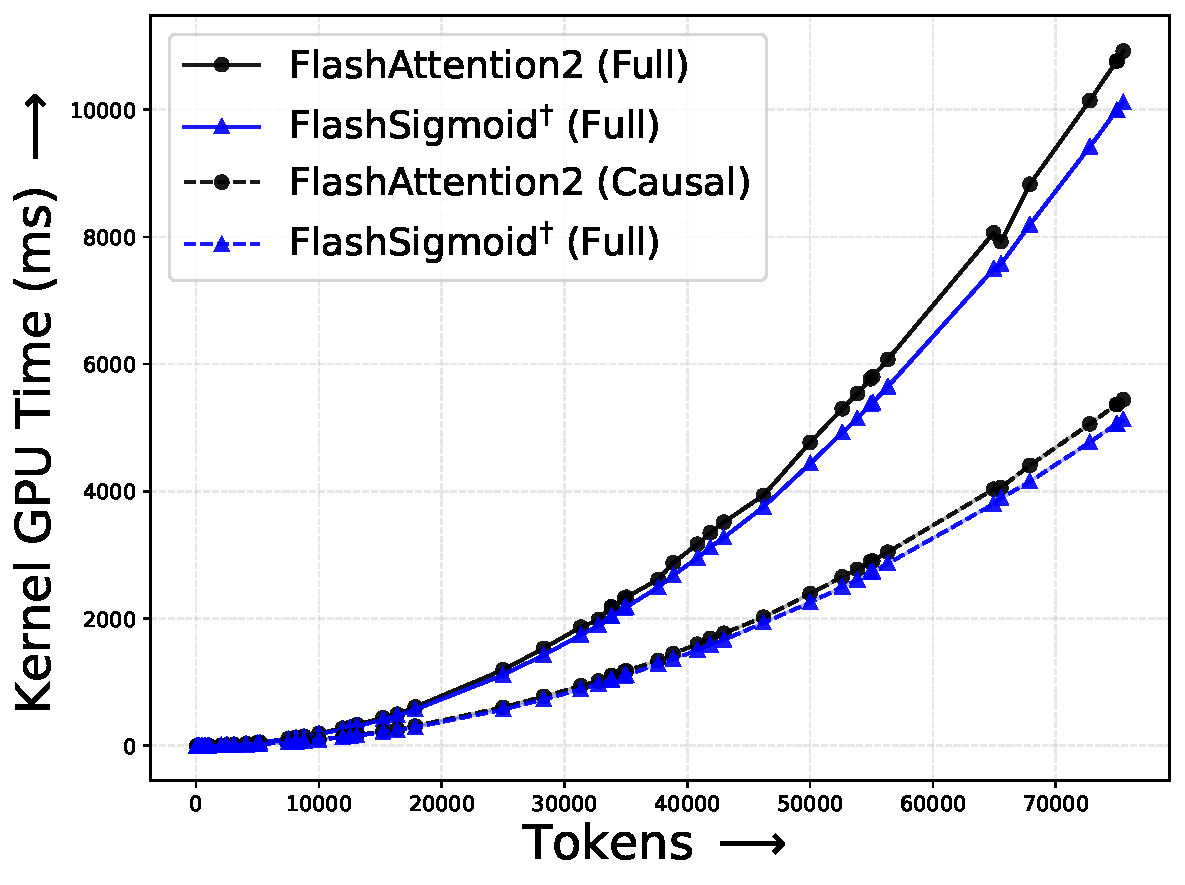
\includegraphics[trim={0 0 0 0}, width=\textwidth]{figures/_flash_figures/final_arxiv/f5/A100_noalibi_FWDBWD_Full_6.18_0.05_Causal_5.76_0.04.pdf}
        \captionsetup{justification=centering} 
        \caption*{
            (b) Training mode kernels on A100.
        }
    \end{minipage}
    \caption{
        On average, for sequence lengths between $[64, 78\mathrm{k}]$, the inference mode kernel of $\textsc{FlashSigmoid}^{\dagger}$ is ${14.82}\%$ faster than \textsc{FlashAttention2} for self-attention and ${18.02}\%$ for causal attention.
        The training mode kernels of $\textsc{FlashSigmoid}^{\dagger}$ are ${6.18}\%$ faster than \textsc{FlashAttention2} for self-attention and ${5.76}\%$ for causal attention.
        Note that inference involves only the forward pass of the model and training involves both the forward and the backward pass of the model. 
    }
    \label{fig:a100-softmax-sigmoid-fwd-bwd-special-variant}
\end{figure}
\vspace{-0.1in}
\begin{table}[htbp]
    \tiny
    \centering
    \begin{sc}
    \resizebox{\columnwidth}{!}{%
    \begin{tabular}{@{\extracolsep{4pt}}ccccc}
        \toprule
            \multirow{2}{*}{Tokens}
            &
            \multicolumn{4}{c}{Kernel GPU Time Comparison}
        \\
        \cmidrule{2-5} 
            & 
            Kernels
            & 
            \textsc{FlashAttention2} (ms)
            & 
            \textsc{FlashSigmoid} (ms)
            & 
            $\textsc{FlashSigmoid}^{\dagger}$ (ms) 
        \\ 
        \toprule
            \multirow{2}{*}{4096} 
            & 
            $\textrm{fwd}$ 
            & 
            $\reading{8.32}{0.02}$
            & 
            $\reading{7.84}{0.03}\ \mathbf{\left(-5.79\%\right)}$
            & 
            $\reading{7.26}{0.02}\ \mathbf{\left(-13.21\%\right)}$
        \\
        \cmidrule{2-5}
            & 
            $\textrm{fwd} + \textrm{bwd}$  
            &  
            $\reading{31.81}{0.08}$
            & 
            $\reading{31.11}{0.08}\ \mathbf{\left(-2.19\%\right)}$
            &  
            $\reading{30.62}{0.09}\ \mathbf{\left(-4.03\%\right)}$
        \\
        \toprule
            \multirow{2}{*}{8100} 
            & 
            $\textrm{fwd}$ 
            & 
            $\reading{33.65}{0.09}$
            & 
            $\reading{27.92}{0.07}\ \mathbf{\left(-17.04\%\right)}$
            & 
            $\reading{28.54}{0.07}\ \mathbf{\left(-15.50\%\right)}$
        \\
        \cmidrule{2-5}
            & 
            $\textrm{fwd} + \textrm{bwd}$  
            & 
            $\reading{128.18}{0.13}$
            & 
            $\reading{119.04}{0.12}\ \mathbf{\left(-7.13\%\right)}$
            & 
            $\reading{119.85}{0.13}\ \mathbf{\left(-6.81\%\right)}$
        \\
        \toprule
            \multirow{2}{*}{10000} 
            & 
            $\textrm{fwd}$ 
            & 
            $\reading{51.17}{0.07}$
            & 
            $\reading{42.49}{0.06}\ \mathbf{\left(-16.96\%\right)}$
            & 
            $\reading{43.53}{0.09}\ \mathbf{\left(-15.32\%\right)}$
        \\
        \cmidrule{2-5} 
            & 
            $\textrm{fwd} + \textrm{bwd}$  
            & 
            $\reading{194.54}{0.14}$
            & 
            $\reading{180.59}{0.15}\ \mathbf{\left(-7.17\%\right)}$
            & 
            $\reading{181.97}{0.17}\ \mathbf{\left(-6.87\%\right)}$
        \\
        \toprule
            \multirow{2}{*}{16384} 
            & 
            $\textrm{fwd}$ 
            & 
            $\reading{134.19}{0.12}$
            & 
            $\reading{125.43}{0.10}\ \mathbf{\left(-6.53\%\right)}$
            & 
            $\reading{116.75}{0.10}\ \mathbf{\left(-13.40\%\right)}$
        \\
        \cmidrule{2-5} 
            & 
            $\textrm{fwd} + \textrm{bwd}$  
            & 
            $\reading{494.65}{0.28}$
            & 
            $\reading{482.08}{0.23}\ \mathbf{\left(-2.54\%\right)}$
            & 
            $\reading{474.52}{0.28}\ \mathbf{\left(-4.48\%\right)}$
        \\
        \bottomrule
        \\
    \end{tabular}
    }
    \caption{
        \textsc{FlashAttention2} vs.
        \textsc{FlashSigmoid} vs. $\textsc{FlashSigmoid}^{\dagger}$ on A100 nodes.
        The kernel GPU time for all three approaches are reported in milliseconds. 
        We observe that $\textsc{FlashSigmoid}^{\dagger}$ provides better and more uniform speed-ups across all example tokens.
    } 
    \label{fig:ComparisonsOfFlashSigmoidVariantsOnA100}
    \end{sc}
\end{table}
\vspace{-0.1in}

\noindent \textbf{Experimentation and Results:}\ For this variant, we perform kernel benchmarking as described in~\cref{sec:PerformanceAnalysisOfFlashSigmoidKernels}, and report the corresponding results in \cref{fig:a100-softmax-sigmoid-fwd-bwd-special-variant}.
Comparing the plots for kernel timing with \textsc{FlashSigmoid} plots from~\cref{fig:a100-softmax-sigmoid-fwd-bwd}, we observe that $\textsc{FlashSigmoid}^{\dagger}$ not only provides a more uniform inference and training kernel speed-up on \emph{all} sequence lengths, but also improves the average of these speed-ups across all lengths.
To further bolster our observations, \cref{fig:ComparisonsOfFlashSigmoidVariantsOnA100} shows the inference mode and training mode kernel speed-ups for a subset of sequence lengths under consideration.
This experiment indicates that it is possible to obtain higher and more uniform speed-ups in kernel timings across a wide range of tokens by investigating optimal block shape, grid shape, and other kernel launch parameters for each input setting and GPU type.
We leave this optimization for future work. 
